\section{Client}

Cette section est entièrement dédiée à la conception du \gls{frontend} de \texttt{SourceCode}. Étant donné qu'il s'agit de la partie visuelle et ergonomique du site, nous aborderons cette thématique de manière plus illustrative.\\

Pour ce faire, nous allons naviguer à travers les différentes pages de la plateforme en expliquant nos choix d'implémentation et les fonctionnalités qui ont été mises en place.\\

Pour vous donner une idée plus claire de ce qui va être abordé, voici une représentation du groupe d'url de premier niveau que contient \texttt{SourceCode}.\\

\begin{figure}[H]
    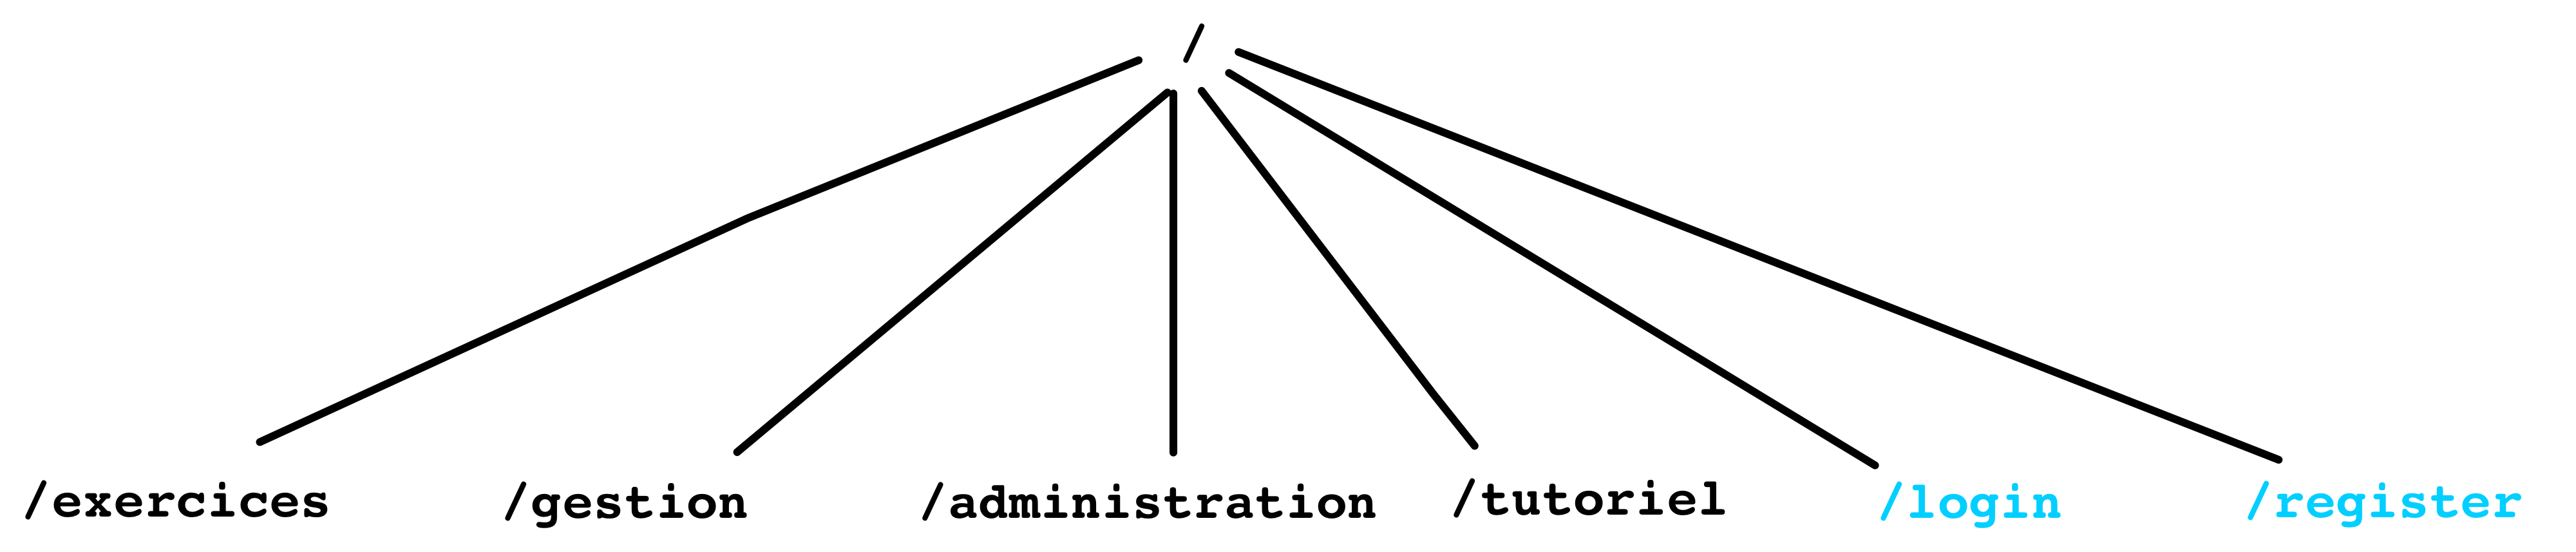
\includegraphics[width=\textwidth,height=0.35\textheight,keepaspectratio]{images/client/overview_client.jpeg}
    \centering
    \caption[SourceCode : Représentation des URL de premier niveau]{URL de premier niveau}
\end{figure}

Cette figure sera notre fil conducteur tout au long de cette section car nous allons analyser chaque url en profondeur. 
Les url en noir signifient qu'elles renferment un niveau supplémentaire d'url tandis que les bleu désignent une page de contenu. Lorsqu'une url contient \textit{\_id}, cela peut être remplacé par un nombre naturel $ n  \epsilon  \mathbb{N} / \{0\}$.\\

L'url \textit{/exercices} représente la bibliothèque de \glspl{resinfo}. C'est dans cet espace que le coeur de \texttt{SourceCode} réside car c'est là que le système de recherche a été pensé pour tout le reste de la plateforme. En outre,
cette même url contient aussi la consultation de \glspl{fiche} lorsque les critères de recherche de l'utilisateur sont satisfaits. À noter que tout type d'utilisateur peut accéder à ces pages.\\

L'url \textit{/gestion} renferme tout ce dont un utilisateur (connecté avec son compte) peut effectuer sur la plateforme pour enrichir son utilisation. On y répertorie la gestion/création/modification de ses propres \glspl{resinfo}, la gestion/création/modification de ses favoris pour faciliter la recherche et enfin, la consultation de son profil. Cette partie est accessible aux utilisateurs et (super-)administrateurs.\\

L'url \textit{/administration} contient les fonctionnalités exigeant le plus haut niveau de privilèges sur \texttt{SourceCode}. Cette partie est donc entièrement dédiée aux administrateurs et super-administrateurs. Ils peuvent gérer absolument toutes les \glspl{resinfo} disponibles sur la plateforme (impliquant aussi la modification et création de celles-ci), l'importation/exportation de \glspl{resinfo}, la gestion/création/modification de \glspl{tag}, la gestion/création/modification des \glspl{tagCat} et finalement la gestion des utilisateurs de la plateforme.\\

L'url \textit{/tutoriel} concerne un aspect plus ludique de \texttt{SourceCode}. Au travers différentes pages, une thématique de l'application est décortiquée afin que l'utilisateur puisse améliorer sa prise en main avec la plateforme.\\

Les deux dernières url de la figure désignent les interfaces de connexion à \texttt{SourceCode} ainsi que la création d'un compte. Nous allons par ailleurs commencer par expliquer celles-ci.\\

\subsection{Connexion et création de compte}

La création d'un compte permet d'accéder à des fonctionnalités supplémentaires comme la création de favoris ou de \glspl{resinfo}.\\

\begin{figure}[H]
    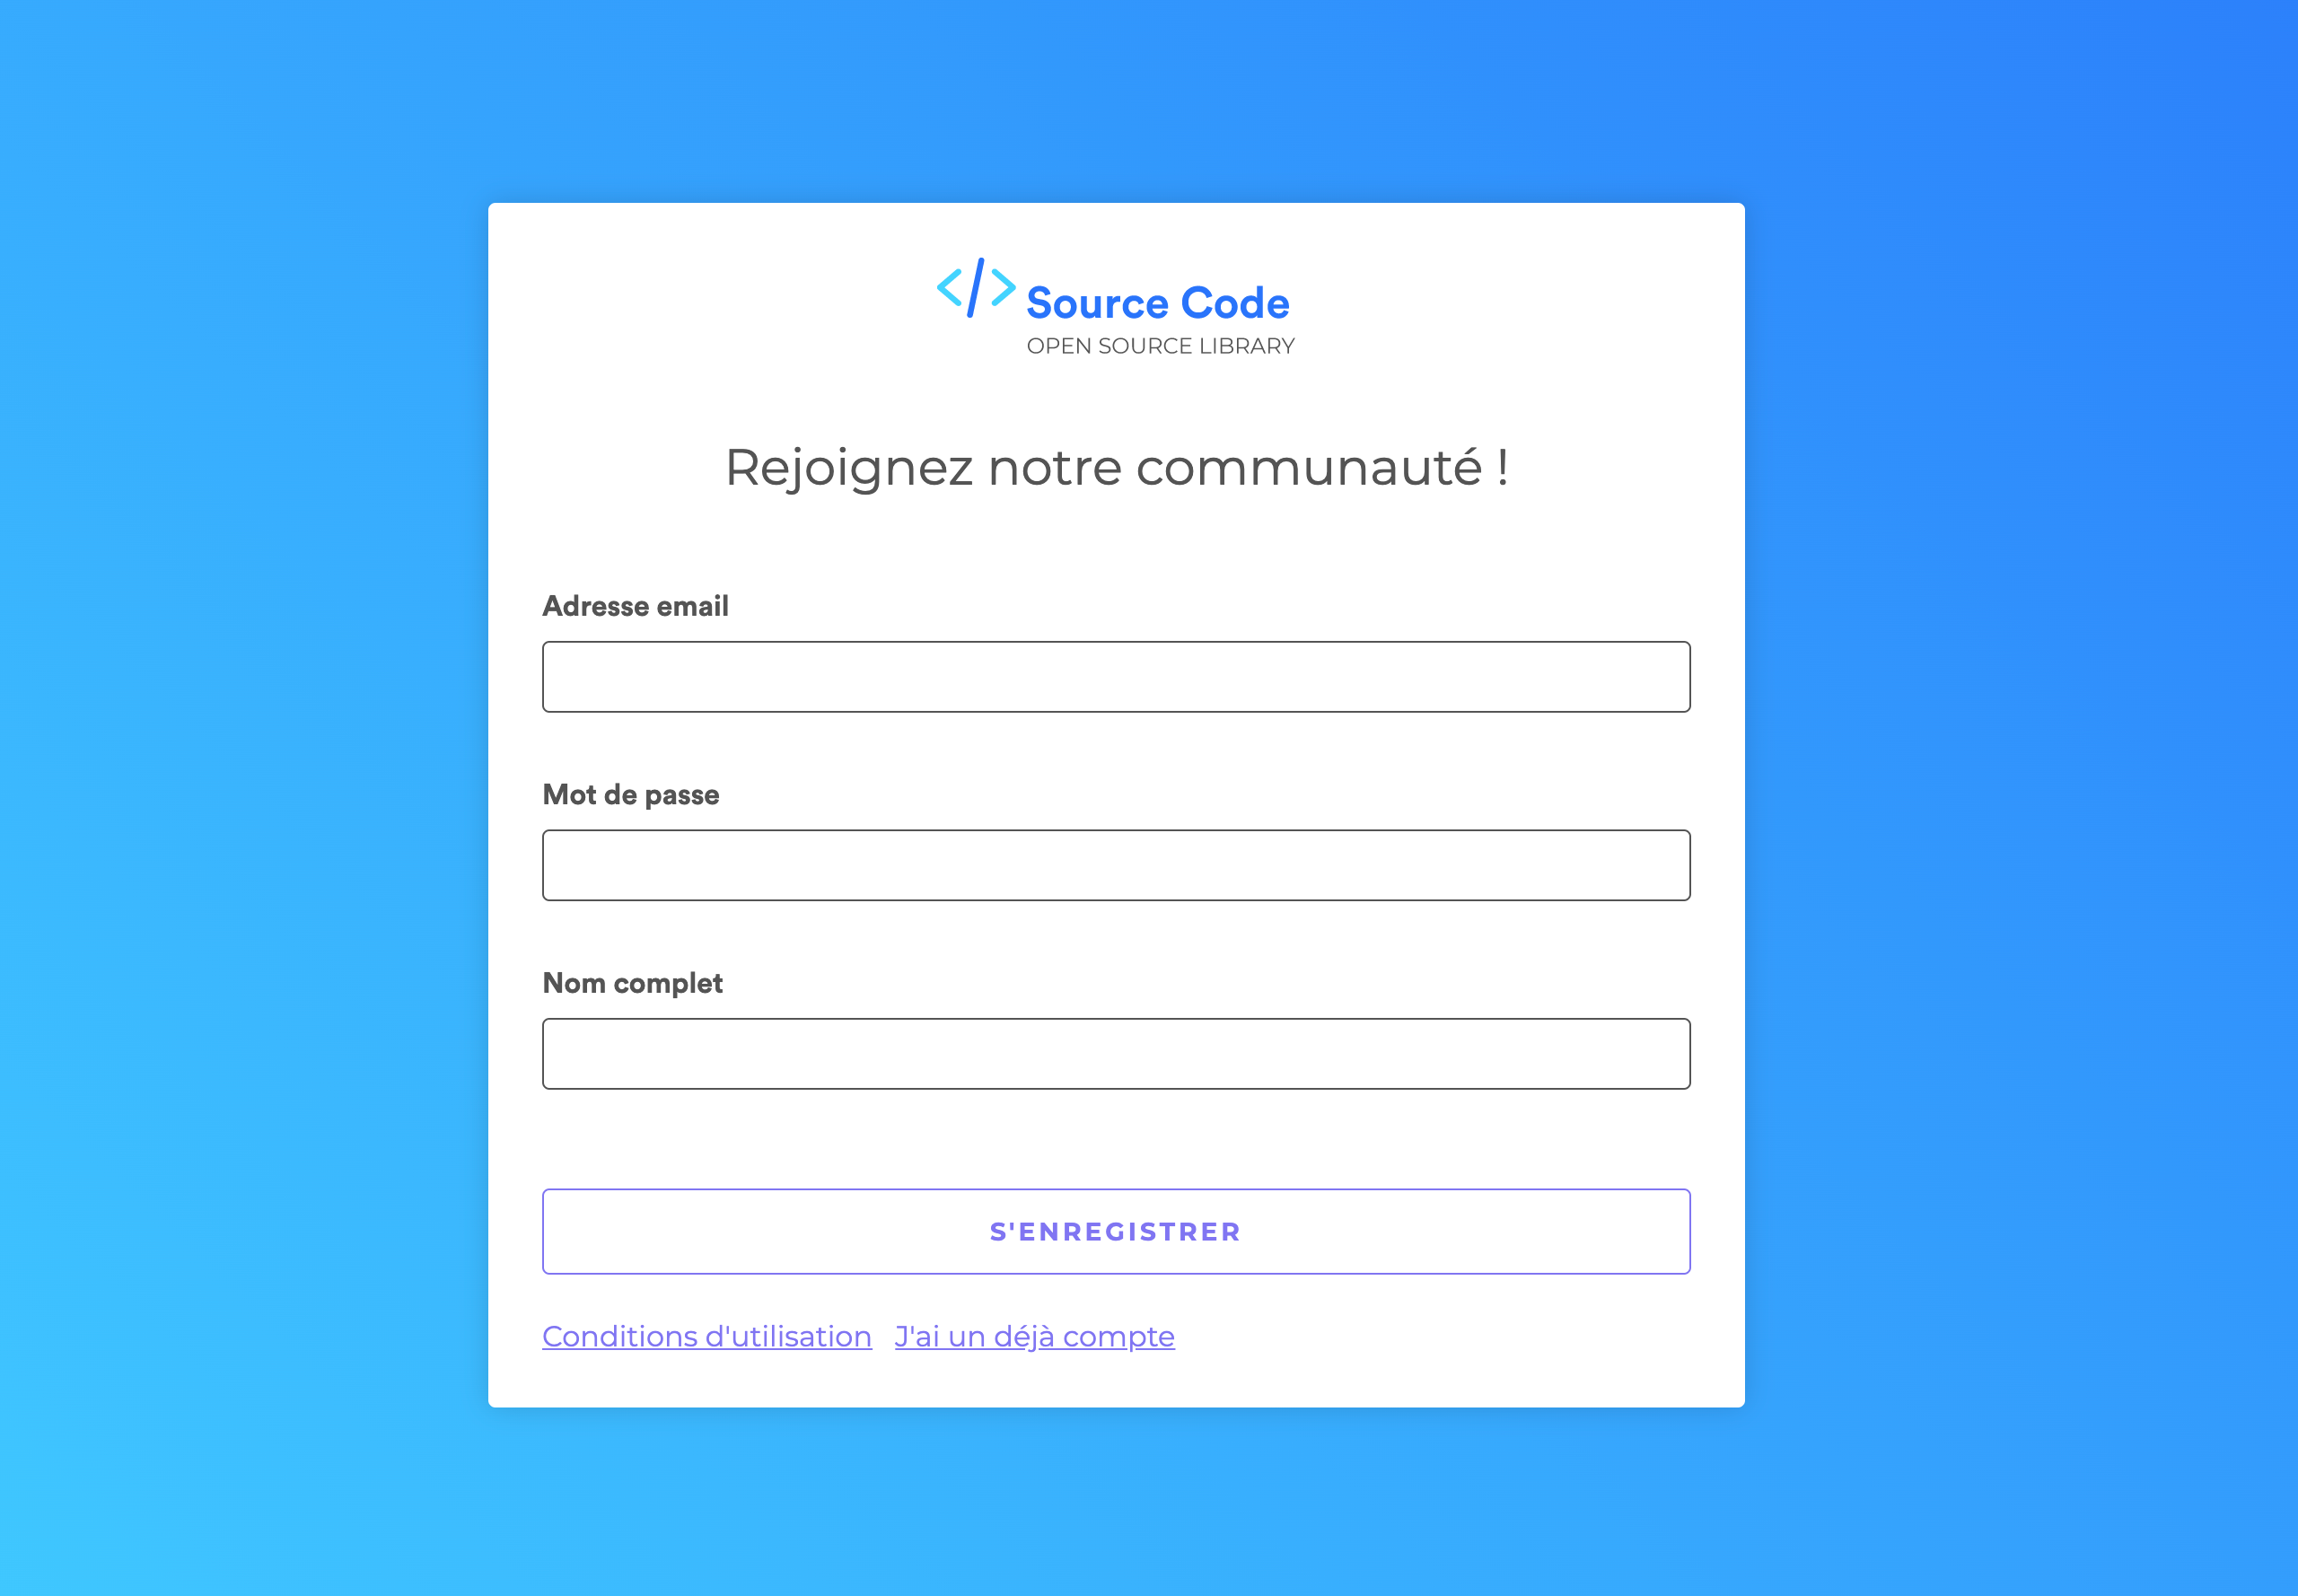
\includegraphics[width=\textwidth,height=0.35\textheight,keepaspectratio]{images/client/register.png}
    \centering
    \caption[SourceCode : interface de création de compte]{Interface de création de compte}
\end{figure}

Par défaut, un compte créé offre les privilèges d'un \textbf{utilisateur}. Voici pour rappel les différents types d'utilisateurs pouvant accéder à la plateforme :

\begin{itemize}
    \item \textbf{Visiteur} : C'est la forme la plus simple. Les droits de ce type d'utilisateur se limitent à la navigation dans la bibliothèque de \glspl{resinfo}. Le système de favoris n'est accessible qu'à partir du moment où vous êtes membre de la plateforme. Nous entendons par là l'utilisateur ou l'administrateur.
    \item \textbf{Utilisateur} : L'utilisateur est membre de l'application. Il possède donc un compte et peut participer au partage de \glspl{resinfo}. L'utilisateur a la possibilité de créer des favoris qu'il pourra ainsi utiliser dans la bibliothèque ou depuis ses interfaces de gestion.
    \item \textbf{(Super-)administrateur} : L'administrateur est un rôle capital car lui seul permet de garantir du contenu de qualité. Il est chargé de valider les \glspl{resinfo} soumises par les utilisateurs, de valider les \glspl{tag} et de créer de nouvelles \glspl{tagCat}. En plus de ces droits-ci, l'administrateur possède bien évidement tous les droits de l'utilisateur !
\end{itemize}

Le formulaire de création nécessite une adresse email (unique), un mot de passe et un nom complet.


\begin{figure}[H]
    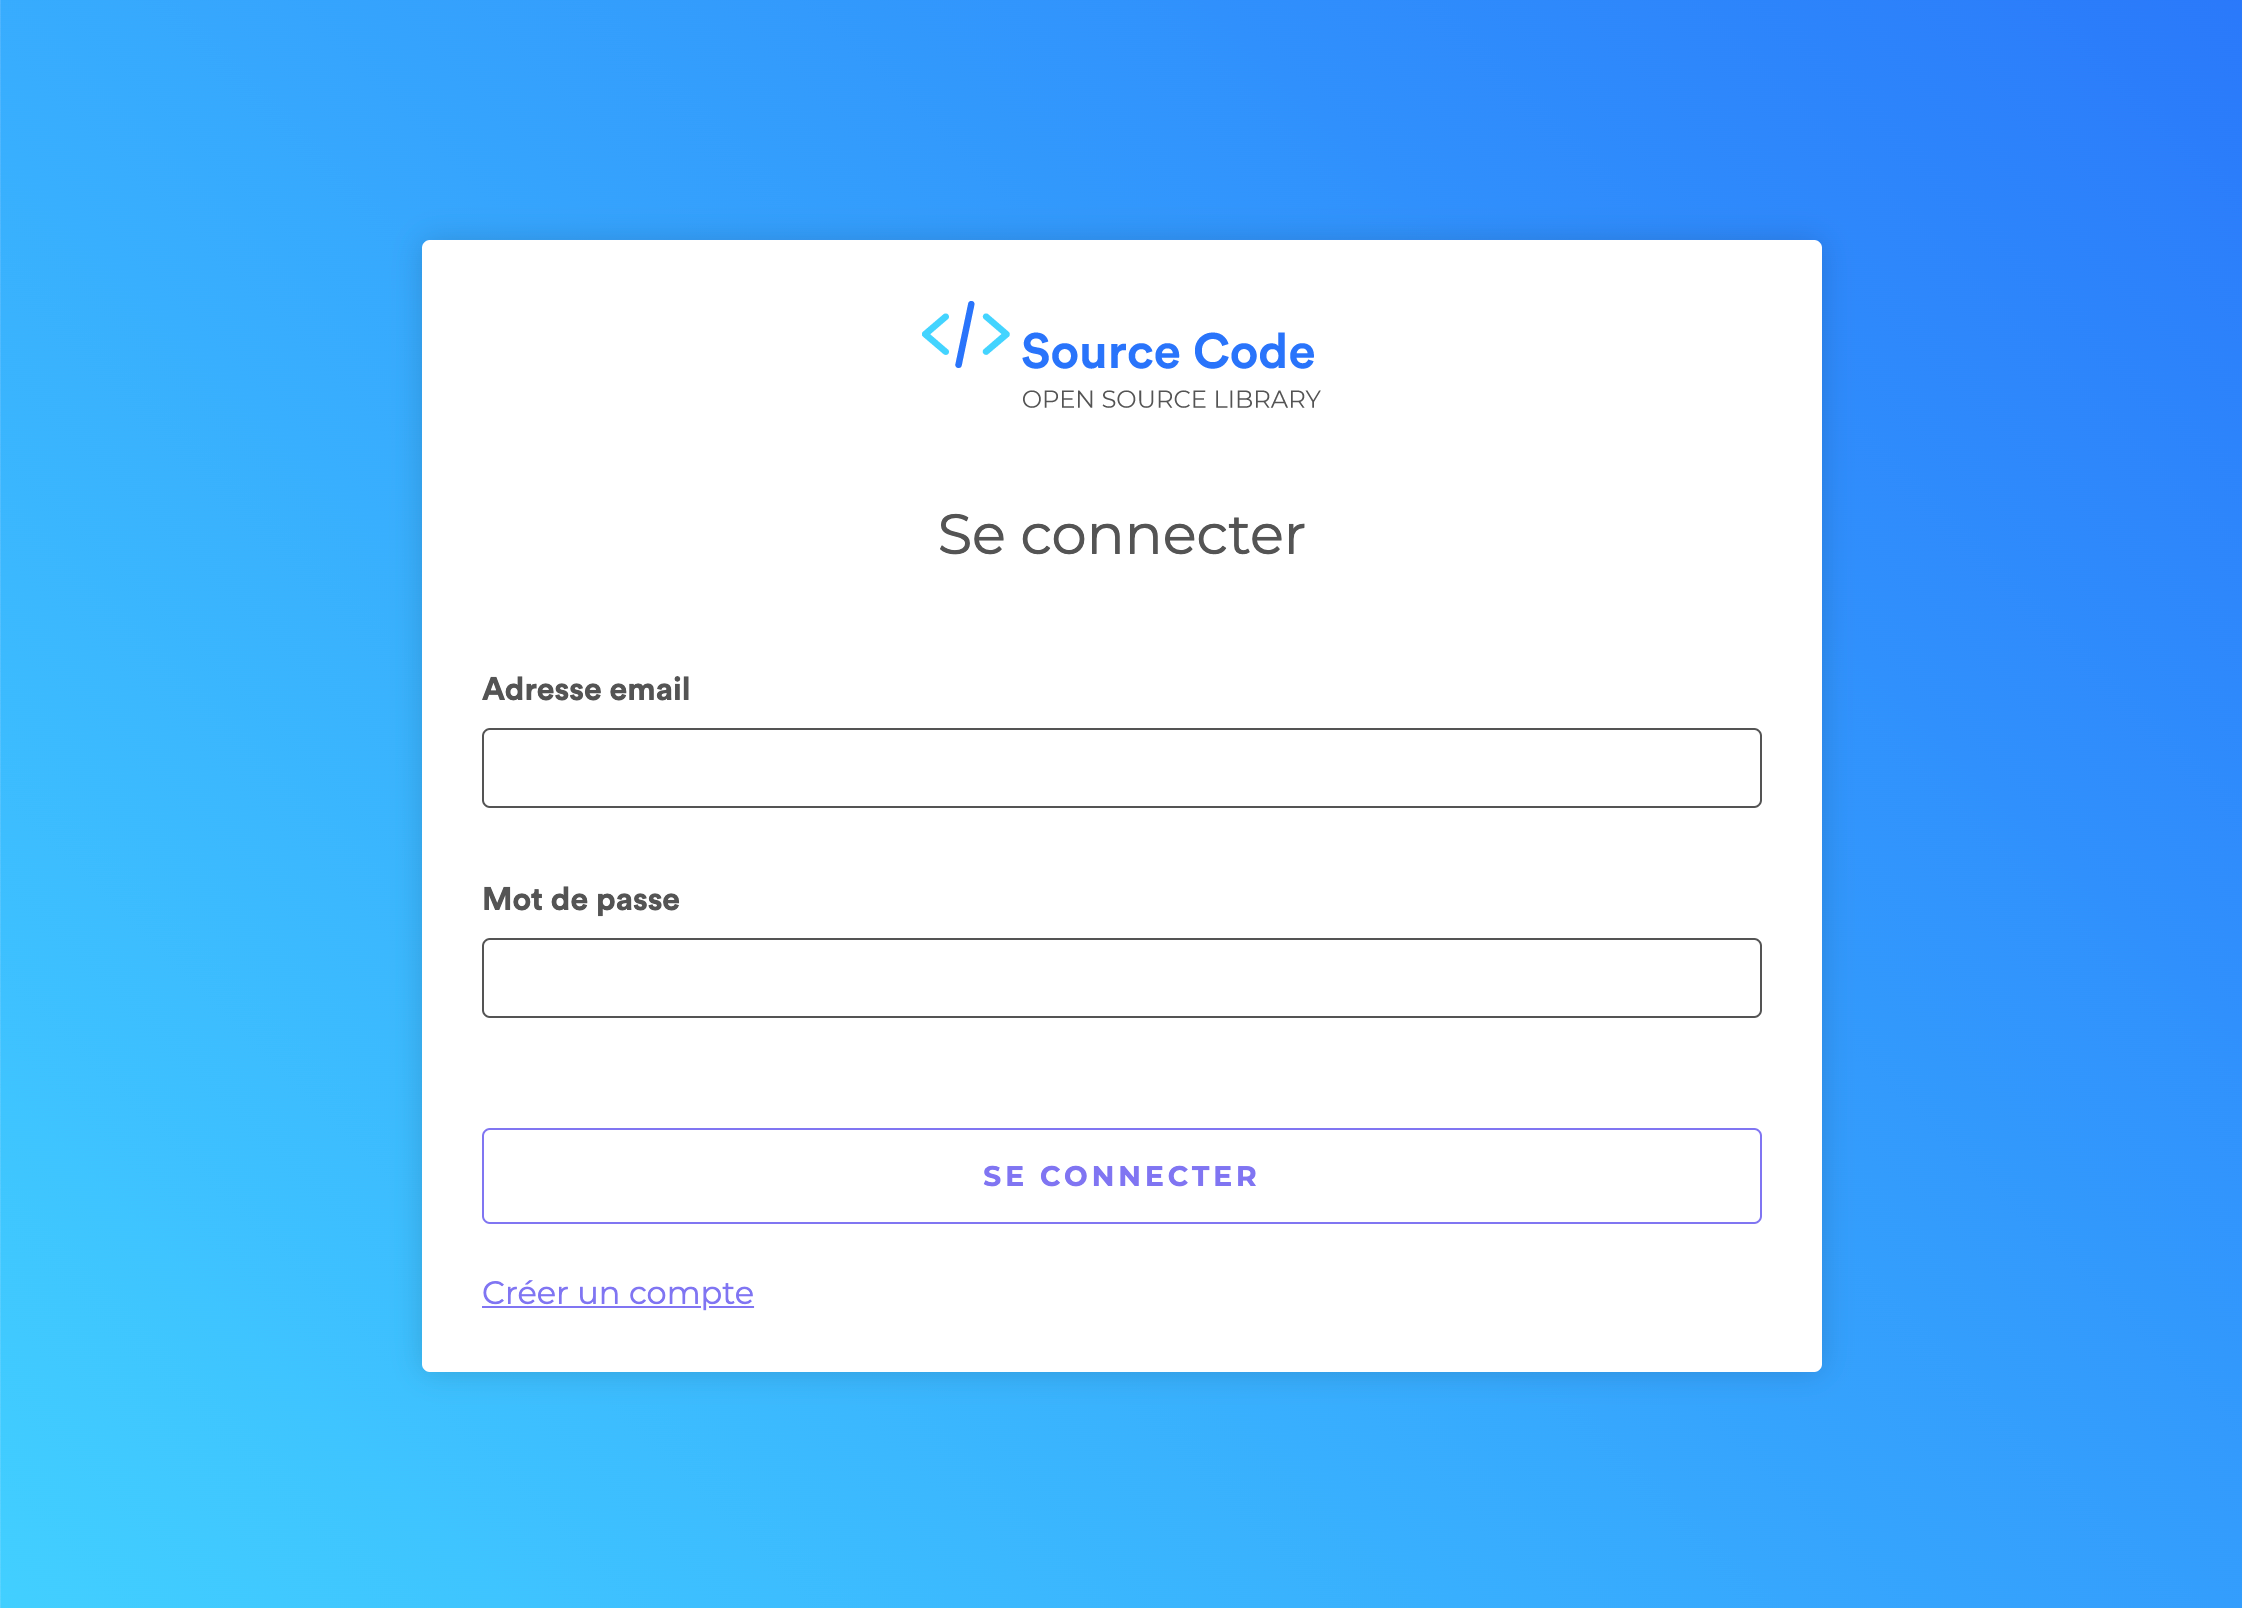
\includegraphics[width=\textwidth,height=0.35\textheight,keepaspectratio]{images/client/login.png}
    \centering
    \caption[SourceCode : interface de connexion]{Interface de connexion}
\end{figure}

Lorsque l'utilisateur possède déjà un compte, il lui suffit de renseigner son adresse email et son mot de passe. Une session d'une heure lui sera attribuée pour gérer ses ressources, favoris,... Après quoi il sera redirigé vers la page de login pour entrer à nouveau ses identifiants.\\


\subsection{Exercices}

La bibliothèque constitue l'élément central de \texttt{SourceCode} pour le partage de ressources. C'est dans cet espace que les \glspl{resinfo} validées par la communauté apparaitront.\\

\begin{figure}[H]
    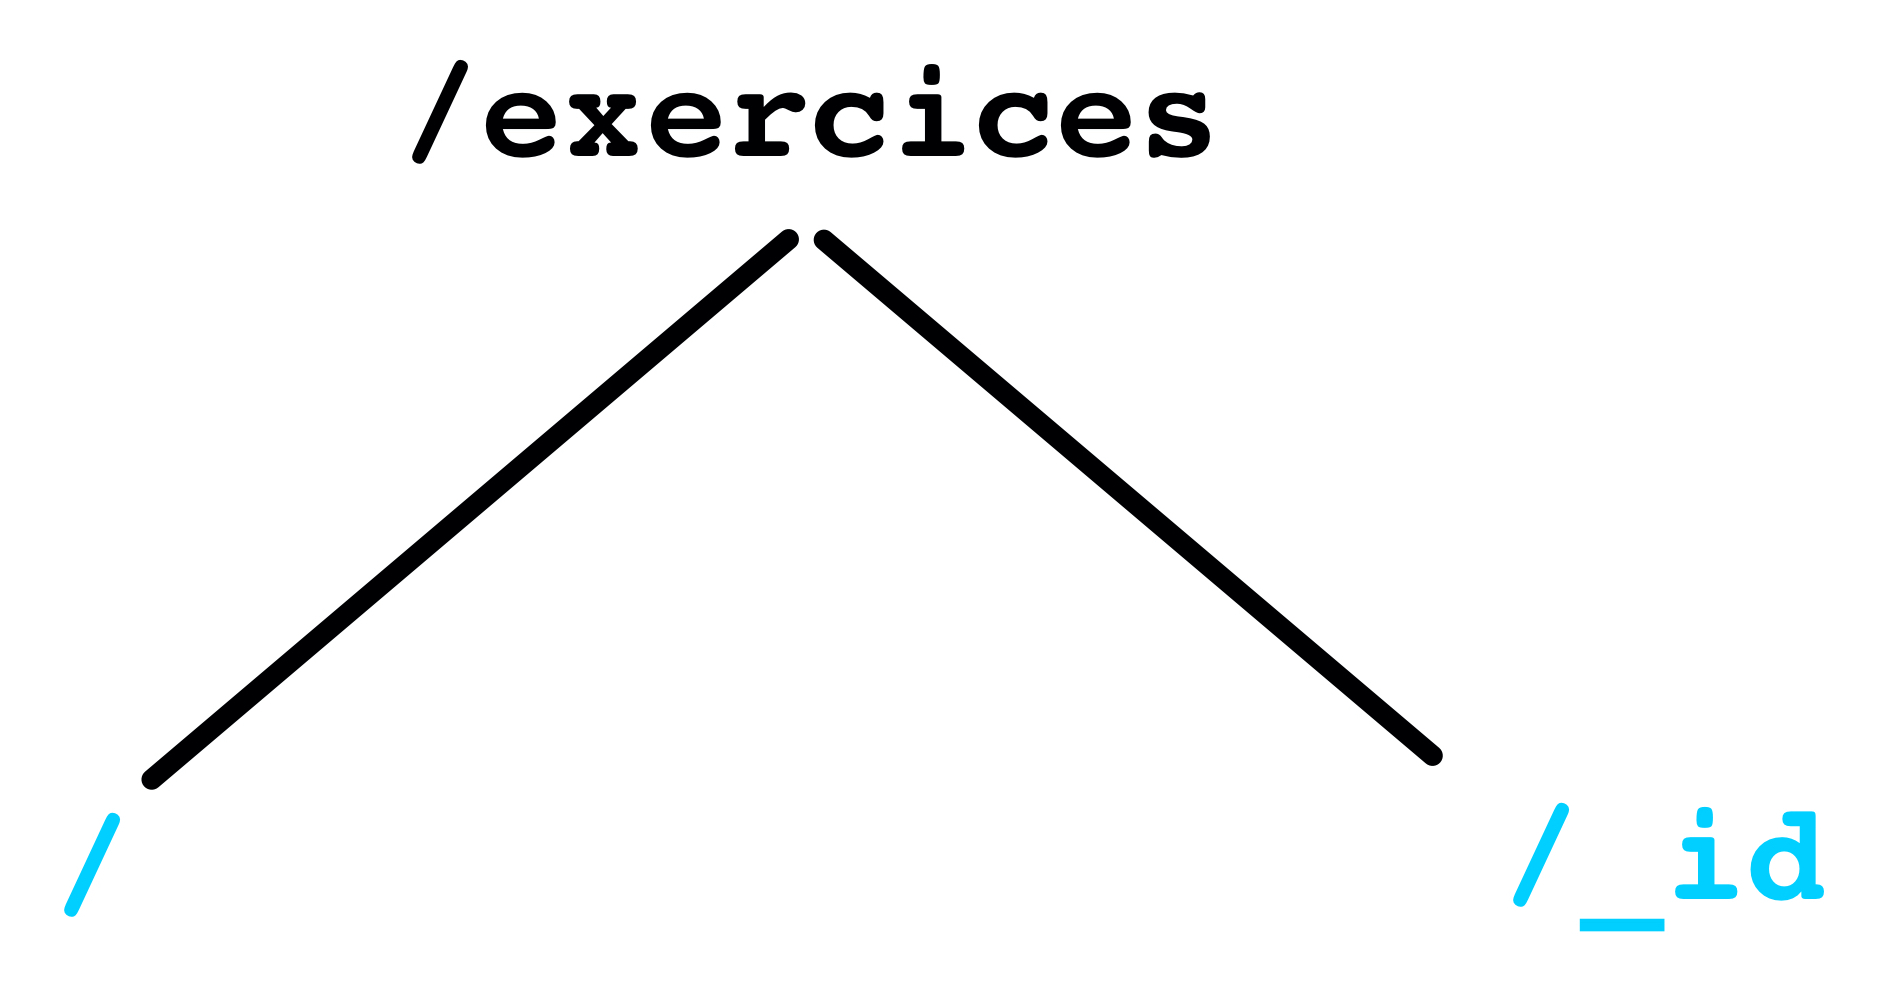
\includegraphics[width=\textwidth,height=0.1\textheight,keepaspectratio]{images/client/exercices.jpeg}
    \centering
    \caption[SourceCode : partie bibliothèque]{Partie bibliothèque (url)}
\end{figure}

Cette section peut se découper en deux parties distinctes :

\begin{itemize}
    \item La bibliothèque, accessible depuis l'url \textit{/exercices}. Nous y aborderons le système de recherche mis en place, les privilèges utilisateurs sur cette page ainsi que les choix ergonomiques.\\
    \item La \gls{fiche} d'une \gls{resinfo}, accessible depuis l'url \textit{/exercices/\_id}. Nous y expliquerons le référencement de la \gls{fiche} afin d'établir un lien avec le fonctionnement de la bibliothèque et comment nous la représentons.
\end{itemize}

\subsubsection{La bibliothèque}

La page \textit{bibliothèque} contient toutes les \glspl{resinfo} ayant été validées par les administrateurs de la plateforme.\\

\begin{figure}[H]
    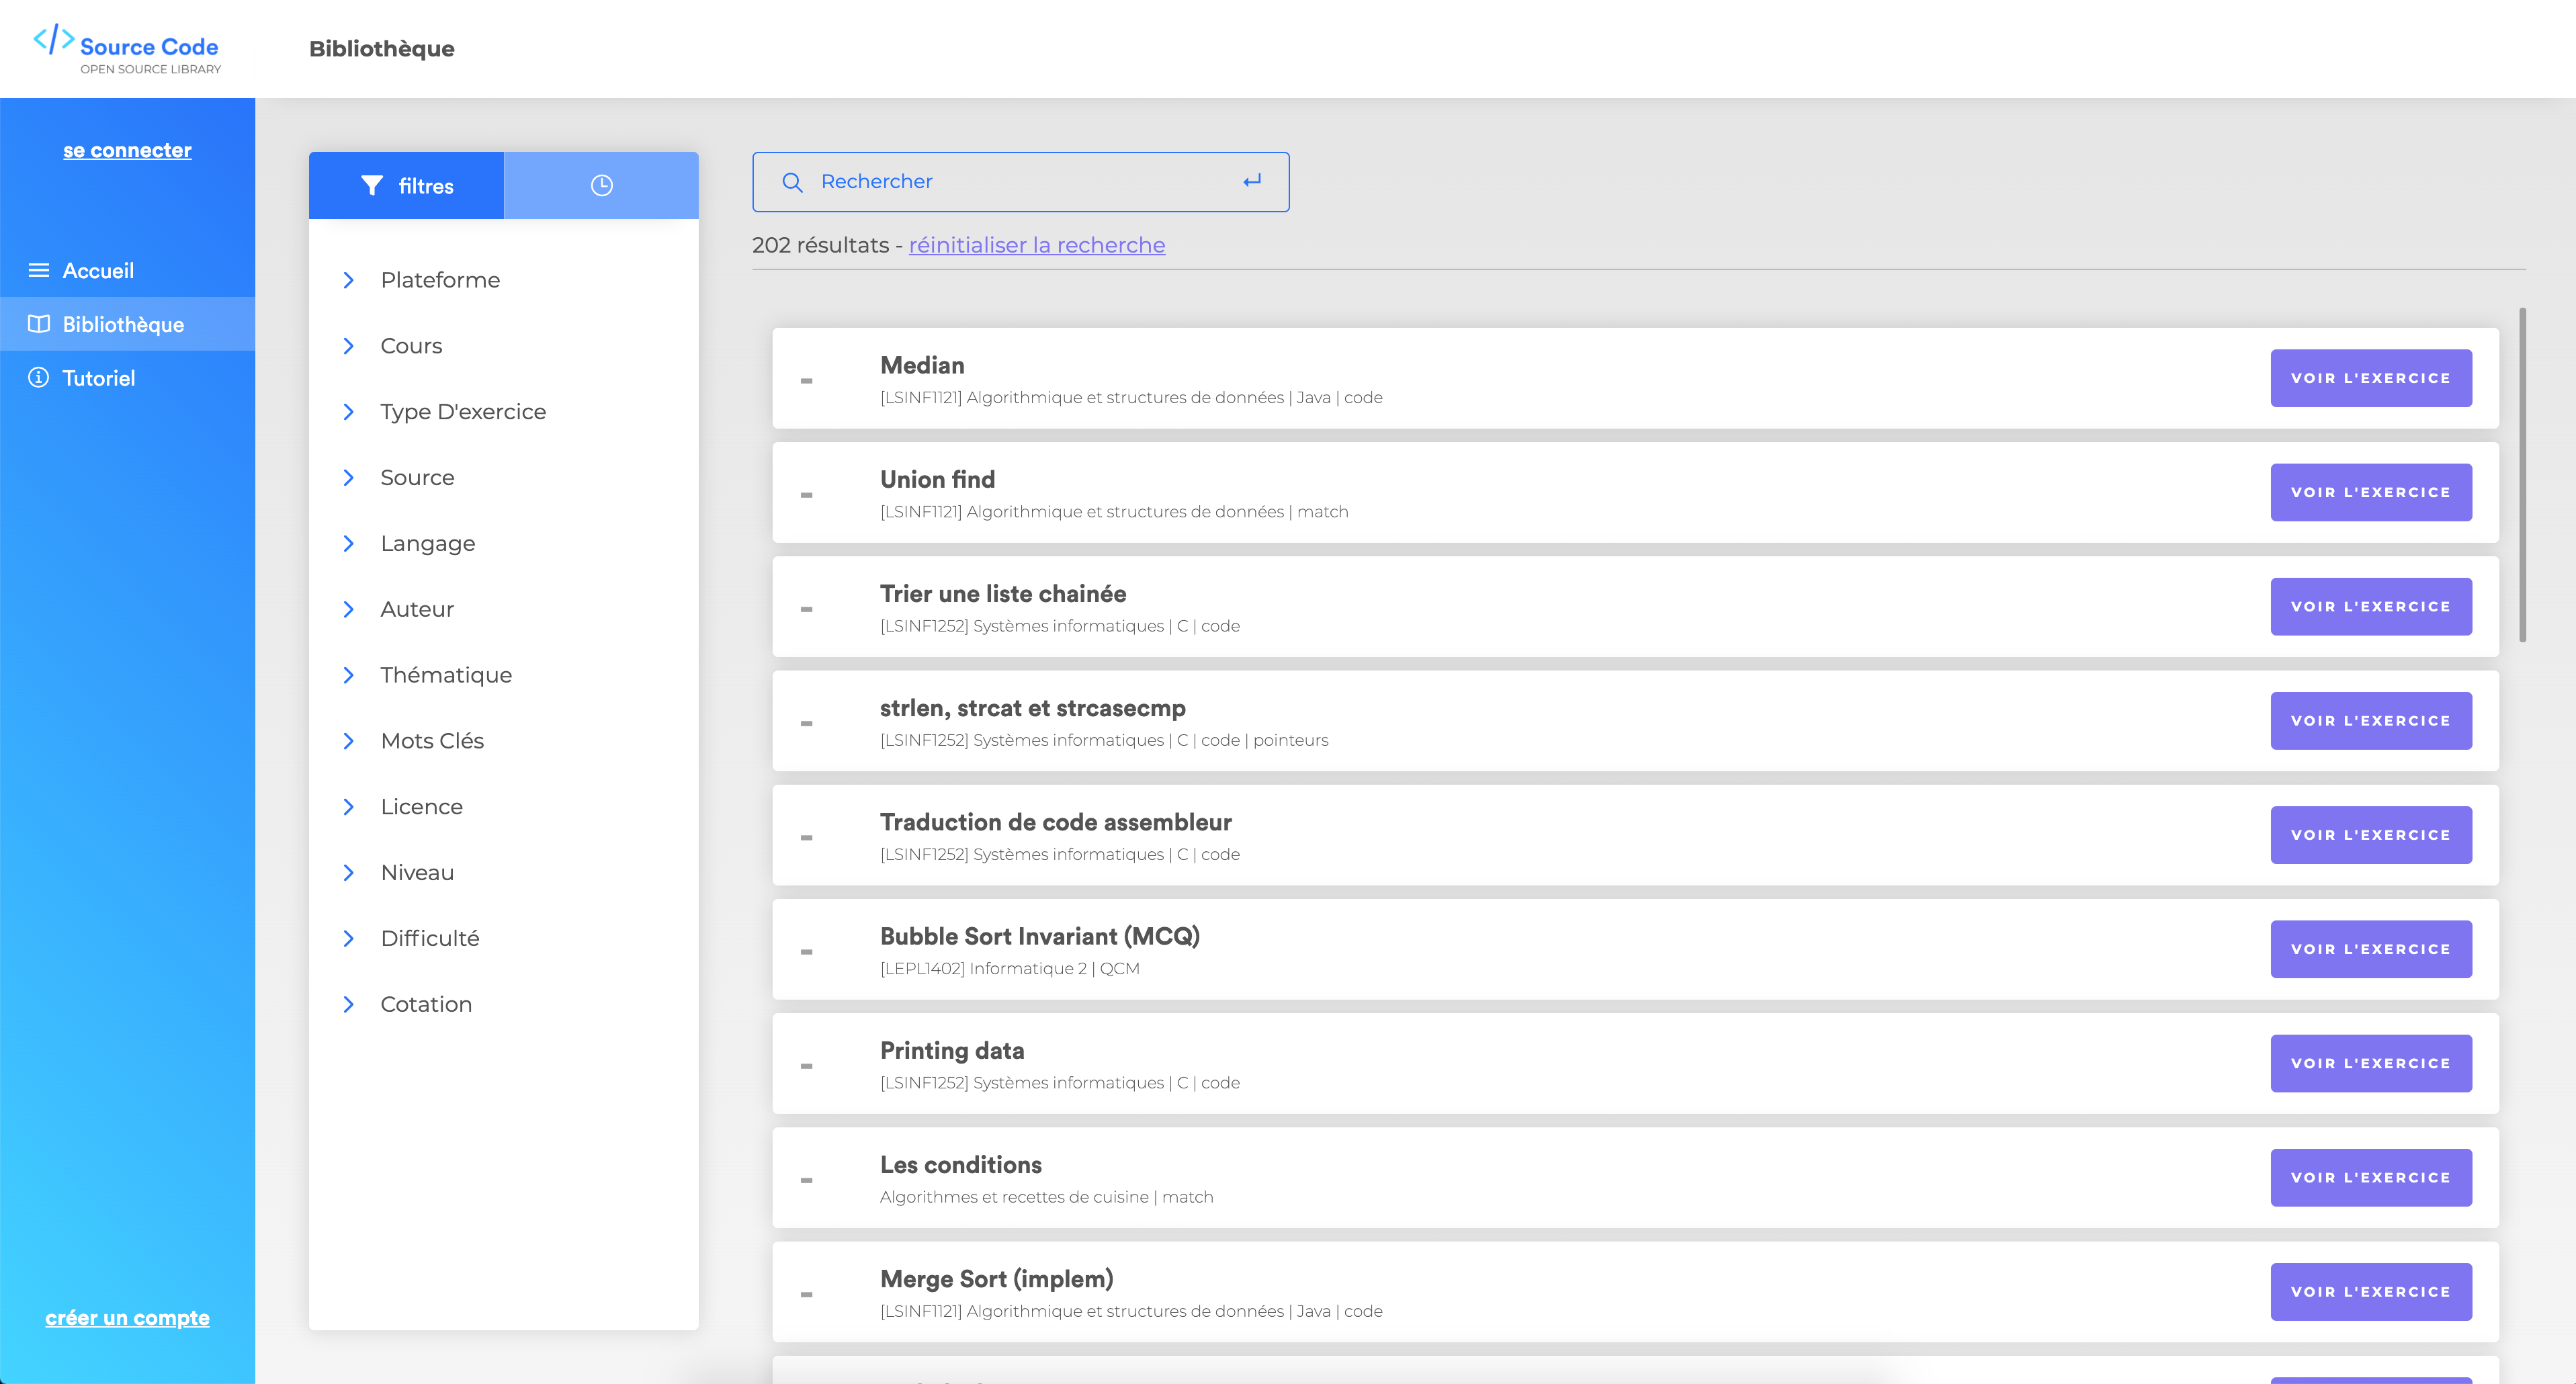
\includegraphics[width=\textwidth,height=\textheight,keepaspectratio]{images/client/library.png}
    \centering
    \caption[SourceCode : page bibliothèque]{page bibliothèque}
\end{figure}


\subsubsubsection*{\textit{Preview d'une \gls{resinfo}}}

La section de droite représente tous les exercices correspondants aux critères de recherche. Il suffit de scroller dans cette section afin de charger les \glspl{resinfo} suivantes.\\

\begin{figure}[H]
    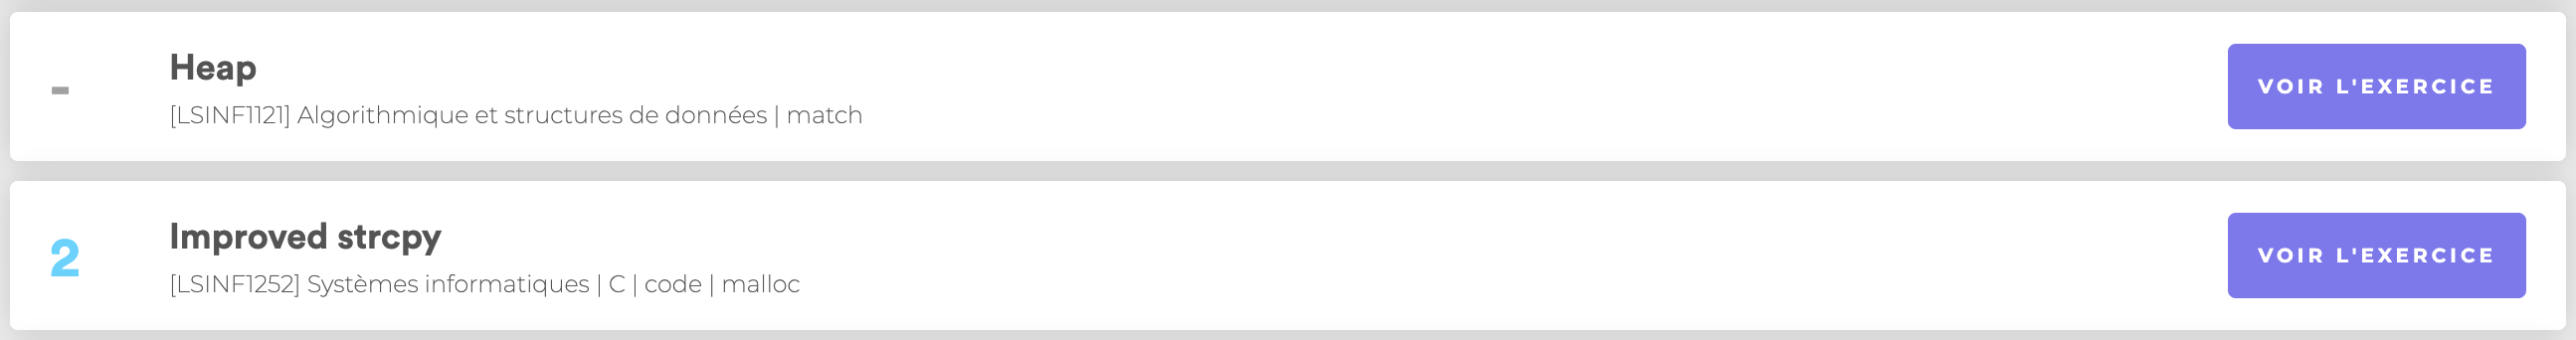
\includegraphics[width=\textwidth,height=\textheight,keepaspectratio]{images/client/preview-exercise.png}
    \centering
    \caption[SourceCode : preview d'une \gls{resinfo}]{Preview d'une \gls{resinfo}}
\end{figure}

La preview d'une ressource contient les informations suivantes :

\begin{itemize}
    \item Le titre de la ressource
    \item Quelques \glspl{tag} pour mieux identifier le type de ressource (si référencés sur celle-ci) : 
    \begin{itemize}
        \item Le cours
        \item Le langage
        \item La difficulté
        \item La thématique
        \item Le type d'exercice
    \end{itemize}
    \item La cotation de la ressource (sur 5)
\end{itemize}

\subsubsubsection*{\textit{Le panneau à onglets}}
\label{section:panneau}

Pour effectuer une recherche dans la bibliothèque, il suffit de taper un titre dans la barre de recherche et/ou d'utiliser le panneau à onglets (élément central de la recherche).\\

Il existe dès lors 3 types d'onglets :

\paragraph{Filtres} permettent d'affiner la recherche de \glspl{resinfo}. Les \glspl{tag} cochés apparaitront juste au-dessus des résultats. Si un \gls{tag} ne convient plus à la recherche, il suffit de décocher un des tags en question ou de cliquer sur la croix du label représentant le \gls{tag} sélectionné.\\

\begin{figure}[H]
    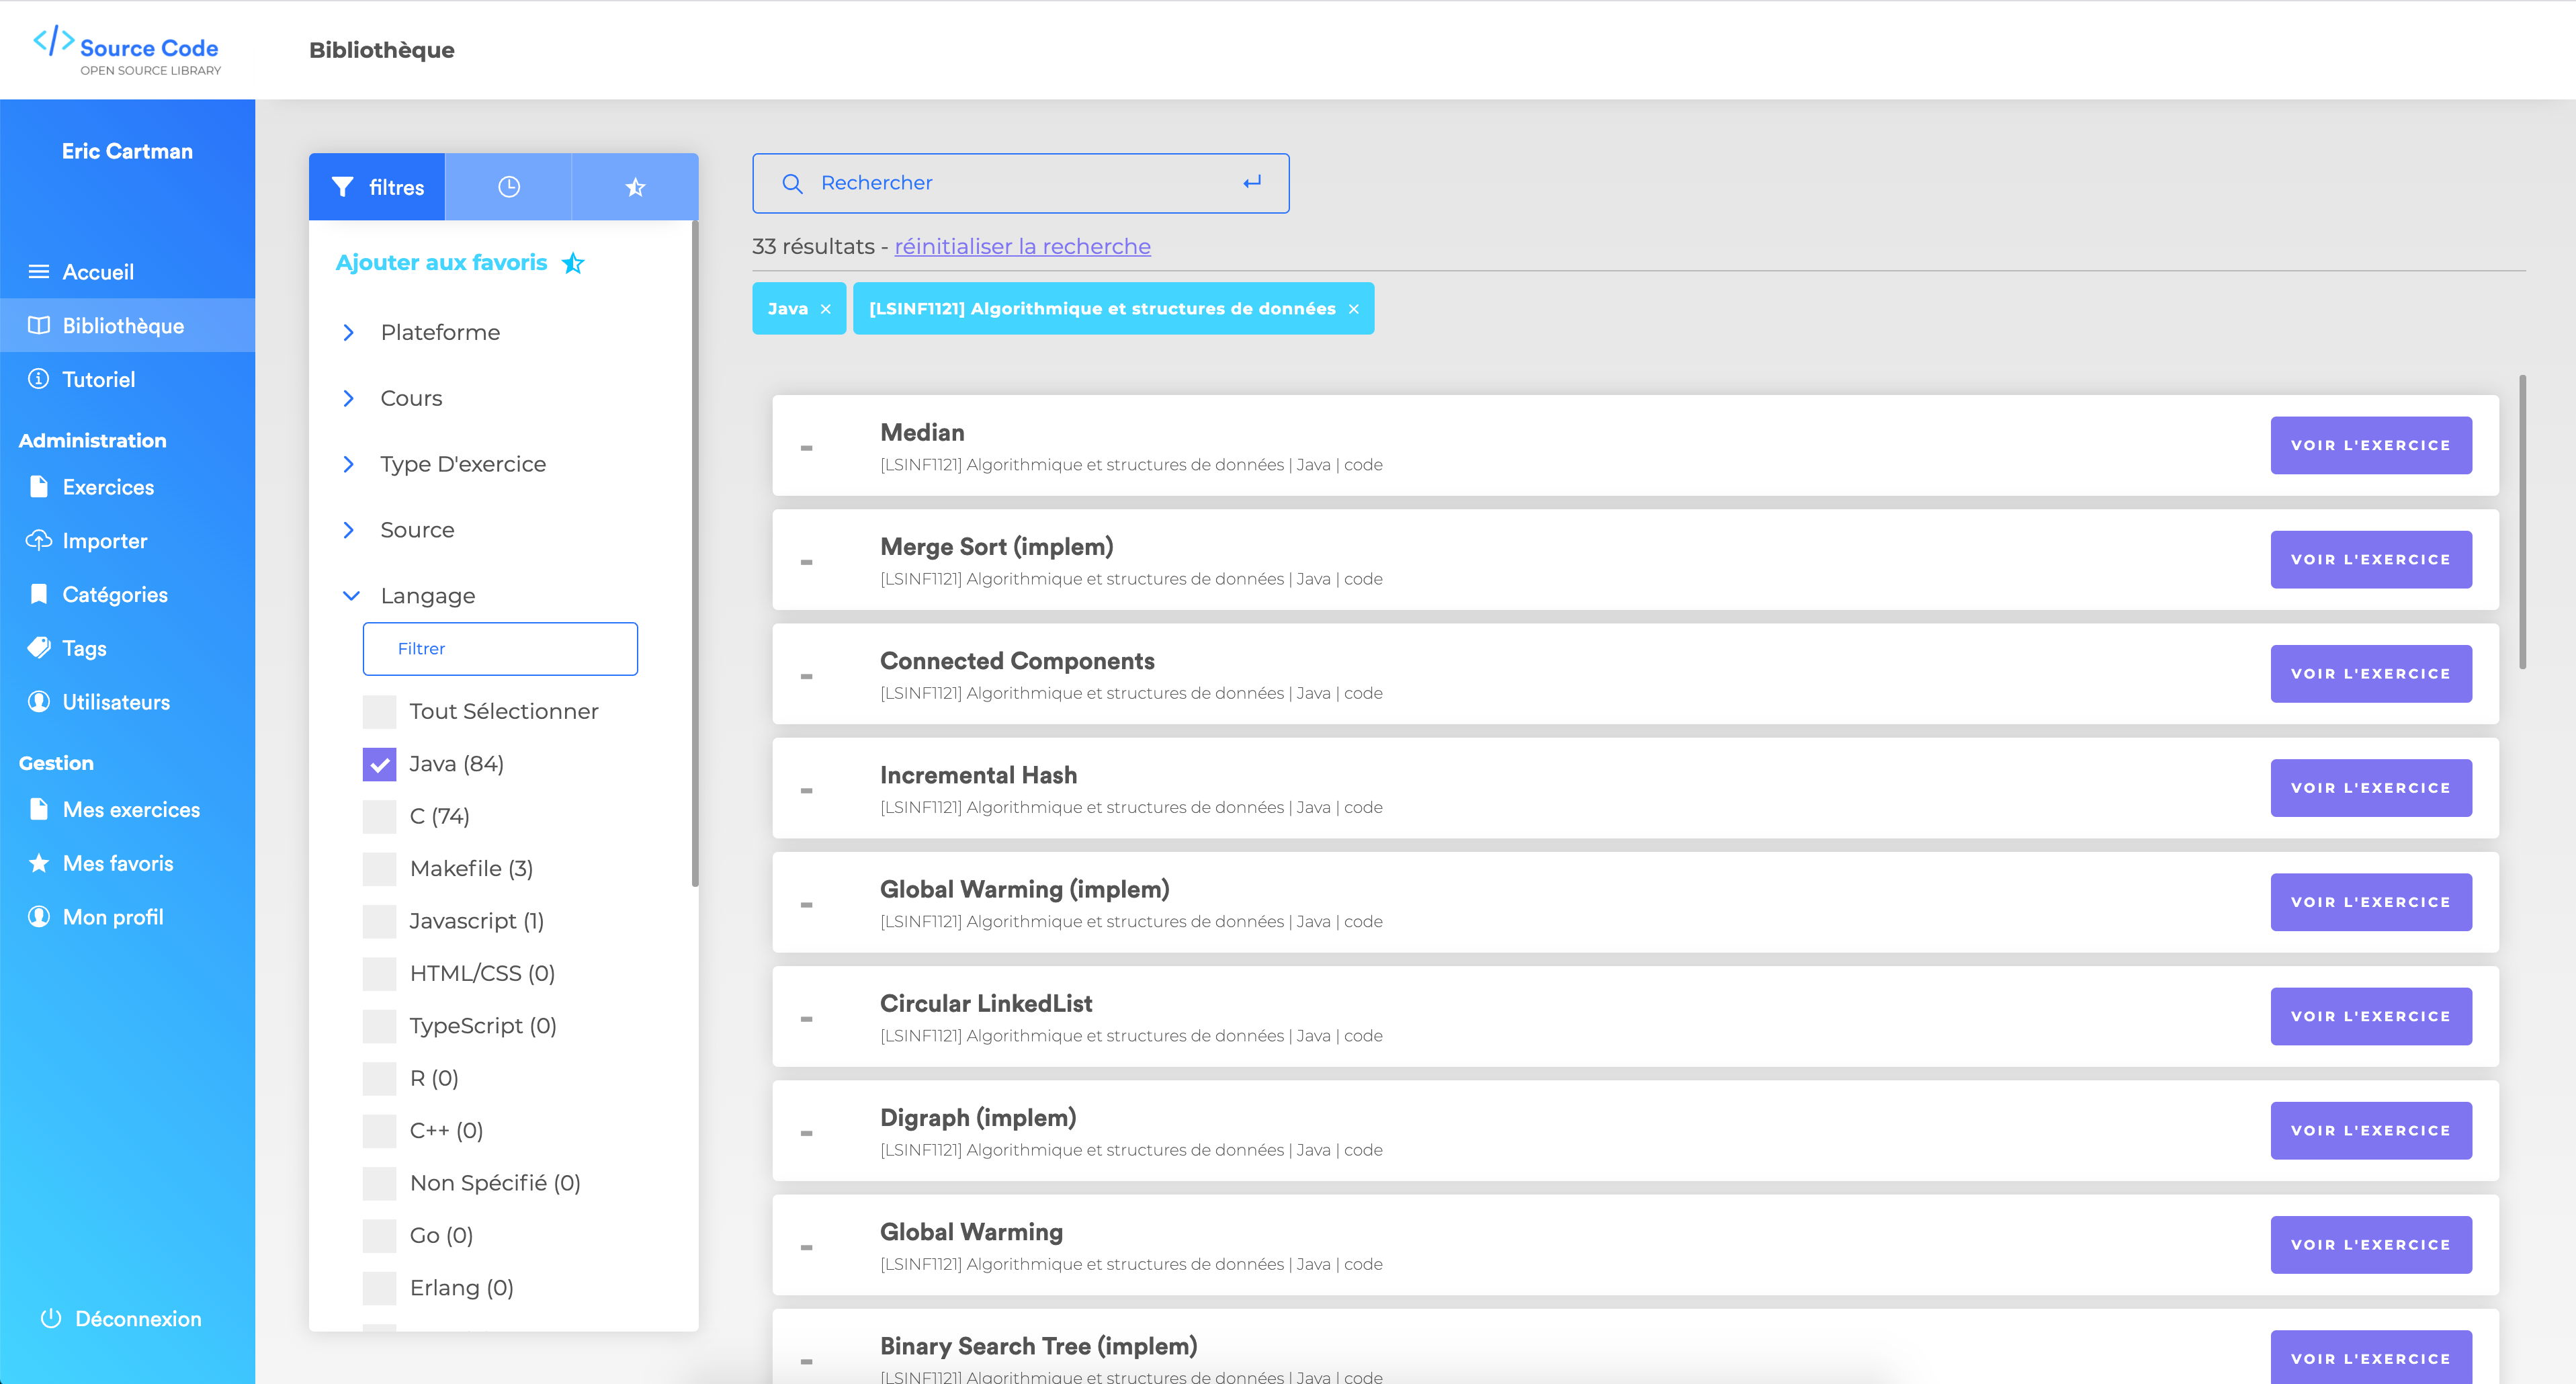
\includegraphics[width=\textwidth,height=\textheight,keepaspectratio]{images/client/search-library.png}
    \centering
    \caption[SourceCode : recherche dans la bibliothèque]{Recherche dans la bibliothèque}
\end{figure}

Plusieurs \glspl{tag} peuvent être choisis dans une même catégorie. Dans ce cas, la recherche donnera des résultats comprenant au moins un des \glspl{tag} sélectionnés.\\

Lorsqu'un \gls{tag} est sélectionné dans deux catégories différentes, la recherche prendra en compte toutes les \glspl{resinfo} comprenant au moins un \gls{tag} sélectionné dans chacune des catégories.\\

\begin{figure}[H]
    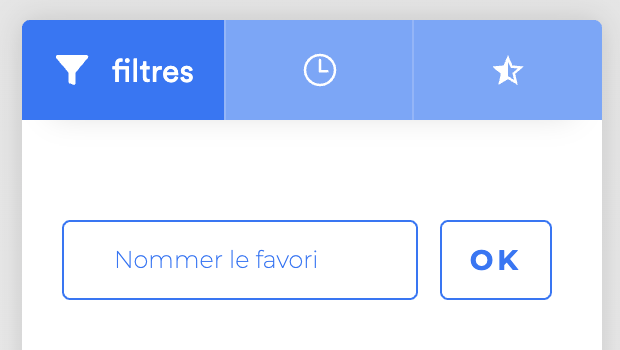
\includegraphics[width=\textwidth,height=0.1\textheight,keepaspectratio]{images/client/add-favorite.png}
    \centering
    \caption[SourceCode : Ajouter aux favoris depuis le panneau "Filtres"]{Ajouter aux favoris depuis le panneau "Filtres"}
\end{figure}

Si vous possédez un compte, vous pouvez enregistrer les critères de recherche actuels en cliquant sur "Ajouter aux favoris". Le texte sera alors remplacé par une entrée texte où le nom de votre favori doit être fourni. Après avoir cliqué sur "Ok", le nouveau favori apparaitra désormais dans l'onglet favoris !\\


\paragraph{Historique} L'historique vous permet de naviguer à travers les recherches que vous avez précédemment effectuées. Il restera disponible tout au long de la session, après quoi il sera réinitialisé.\\

\begin{figure}[H]
    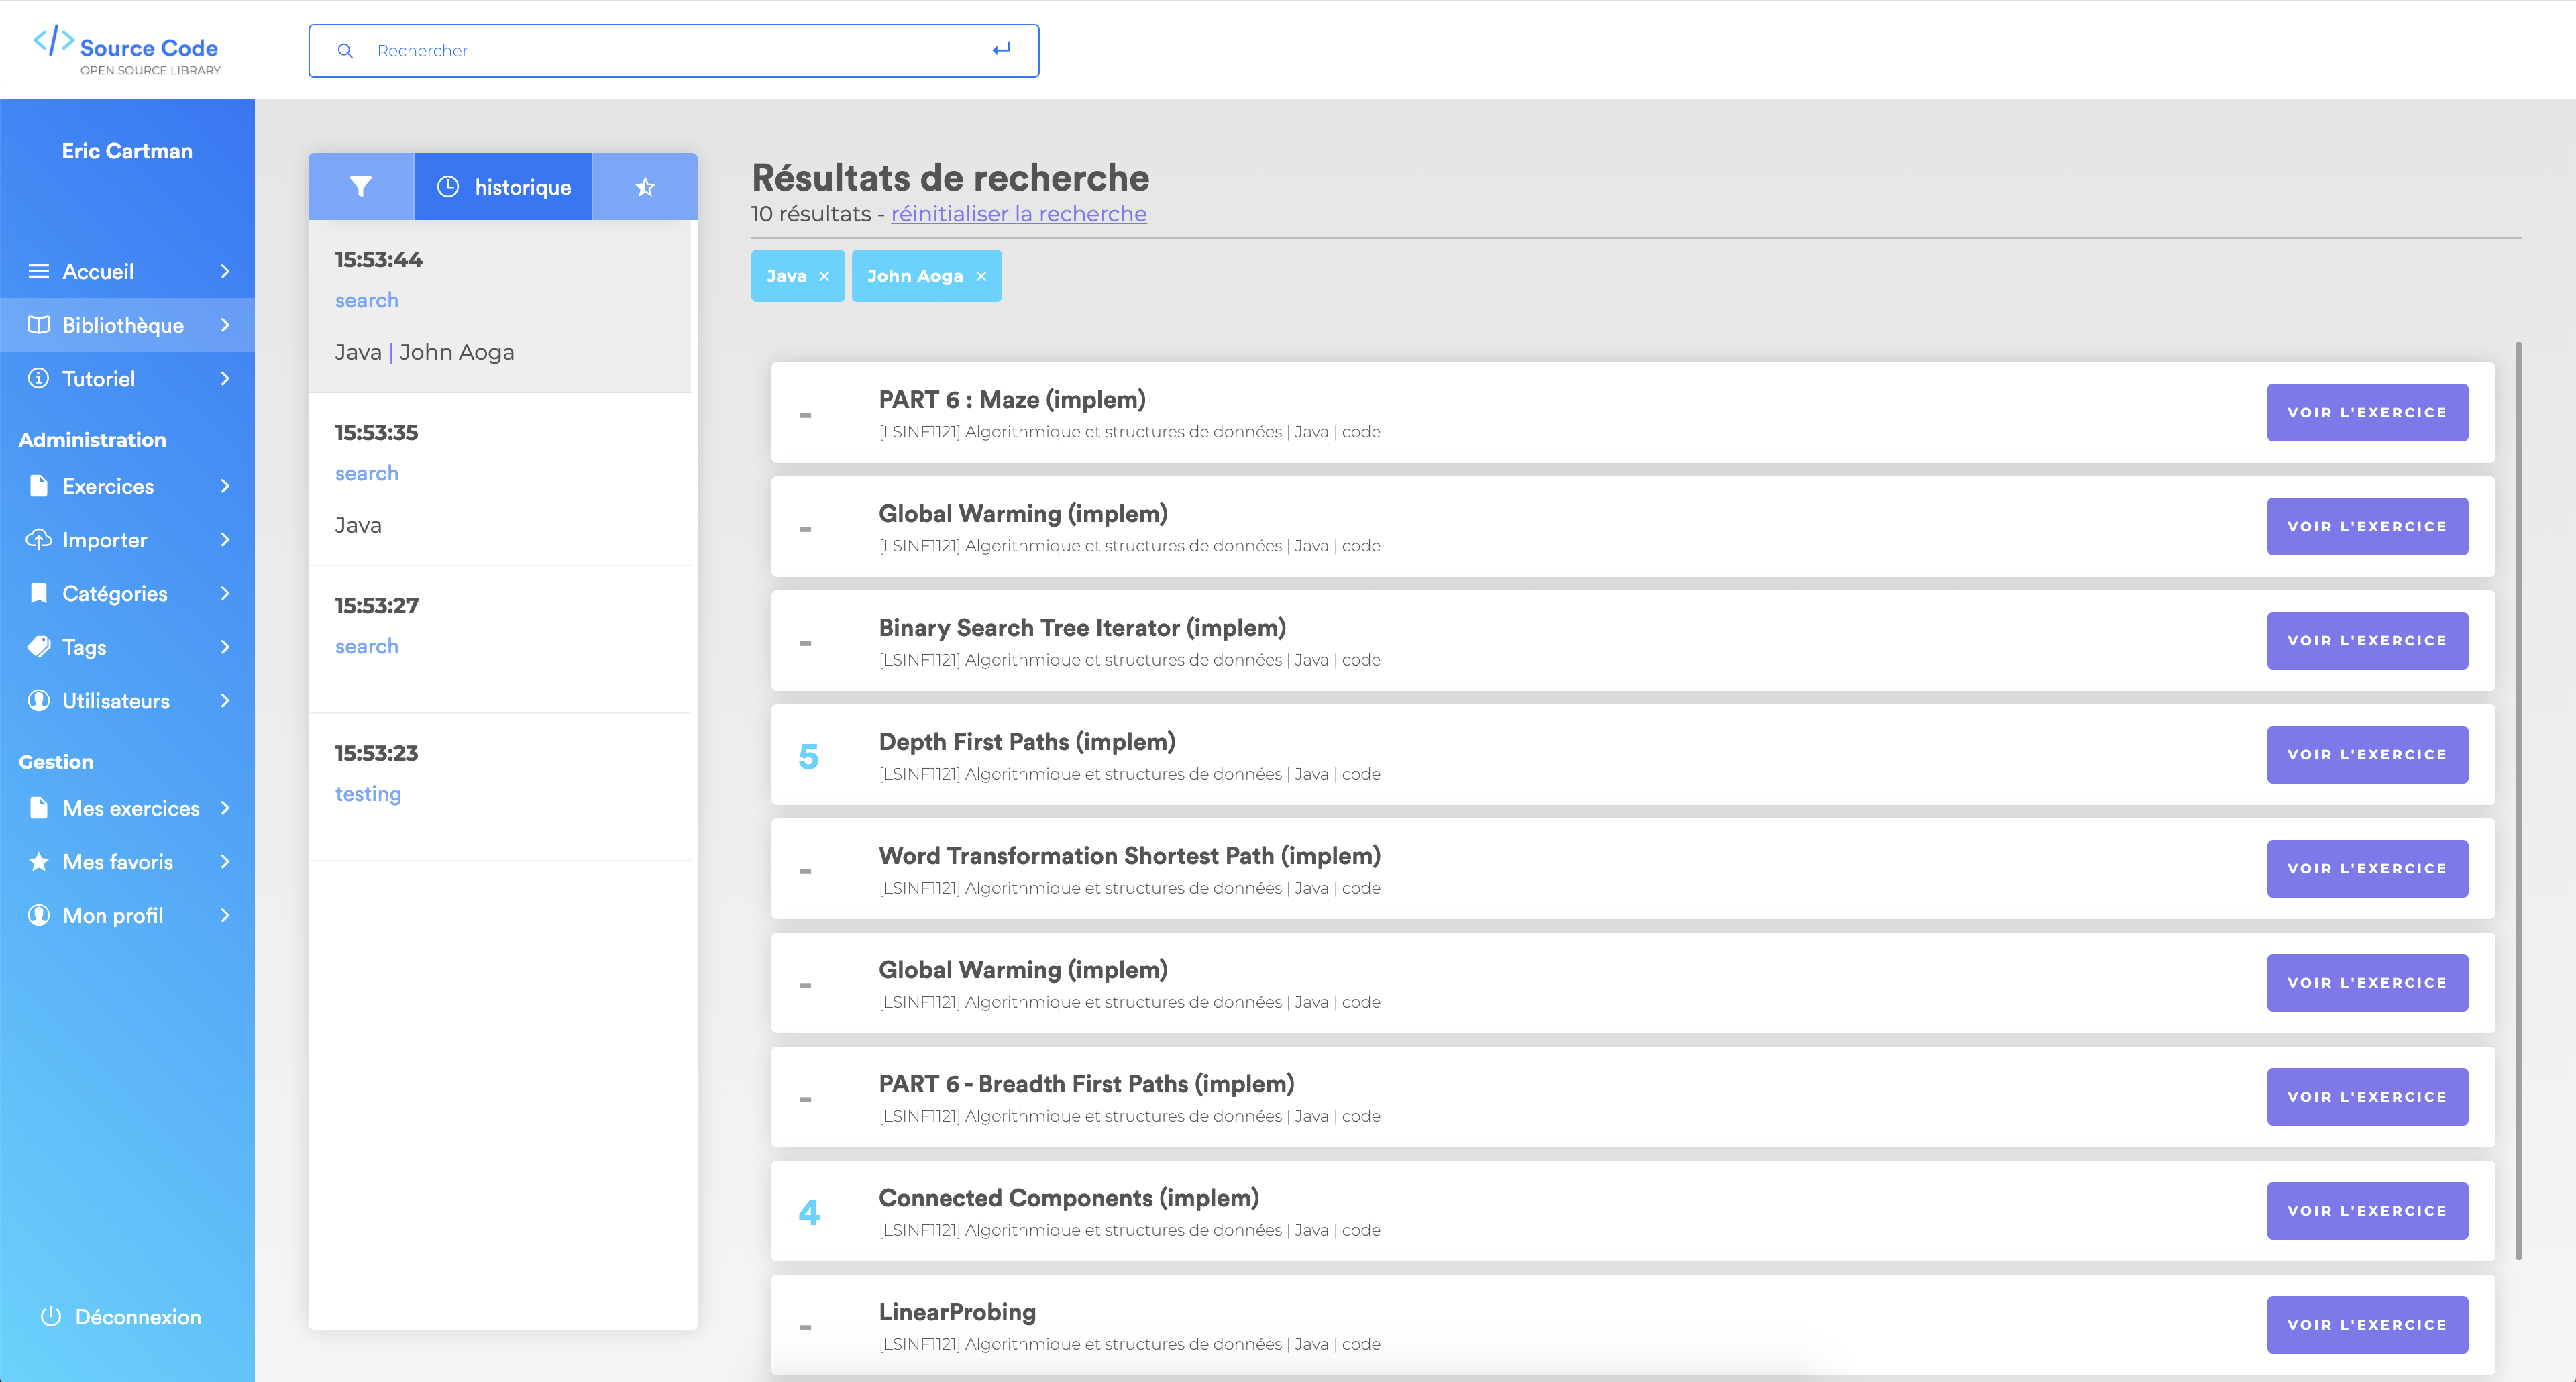
\includegraphics[width=\textwidth,height=\textheight,keepaspectratio]{images/client/historical.png}
    \centering
    \caption[SourceCode : le panneau "Historique"]{Le panneau "Historique"}
\end{figure}

L'historique affiche les recherches précédemment effectuées, de la plus récente à la plus ancienne. Le titre de votre recherche s'affichera en bleu tandis que les \glspl{tag} sélectionnés seront affichés en mode "pêle-mêle", séparés par une barre verticale (|).\\

\paragraph{Favoris (seulement lorsqu'on est connecté !)} Les favoris précédemment créés apparaitront dans ce panneau. Pour utiliser un de des favoris, il suffit de cliquer sur l'un d'eux et la recherche s'actualisera depuis la même page.

\begin{figure}[H]
    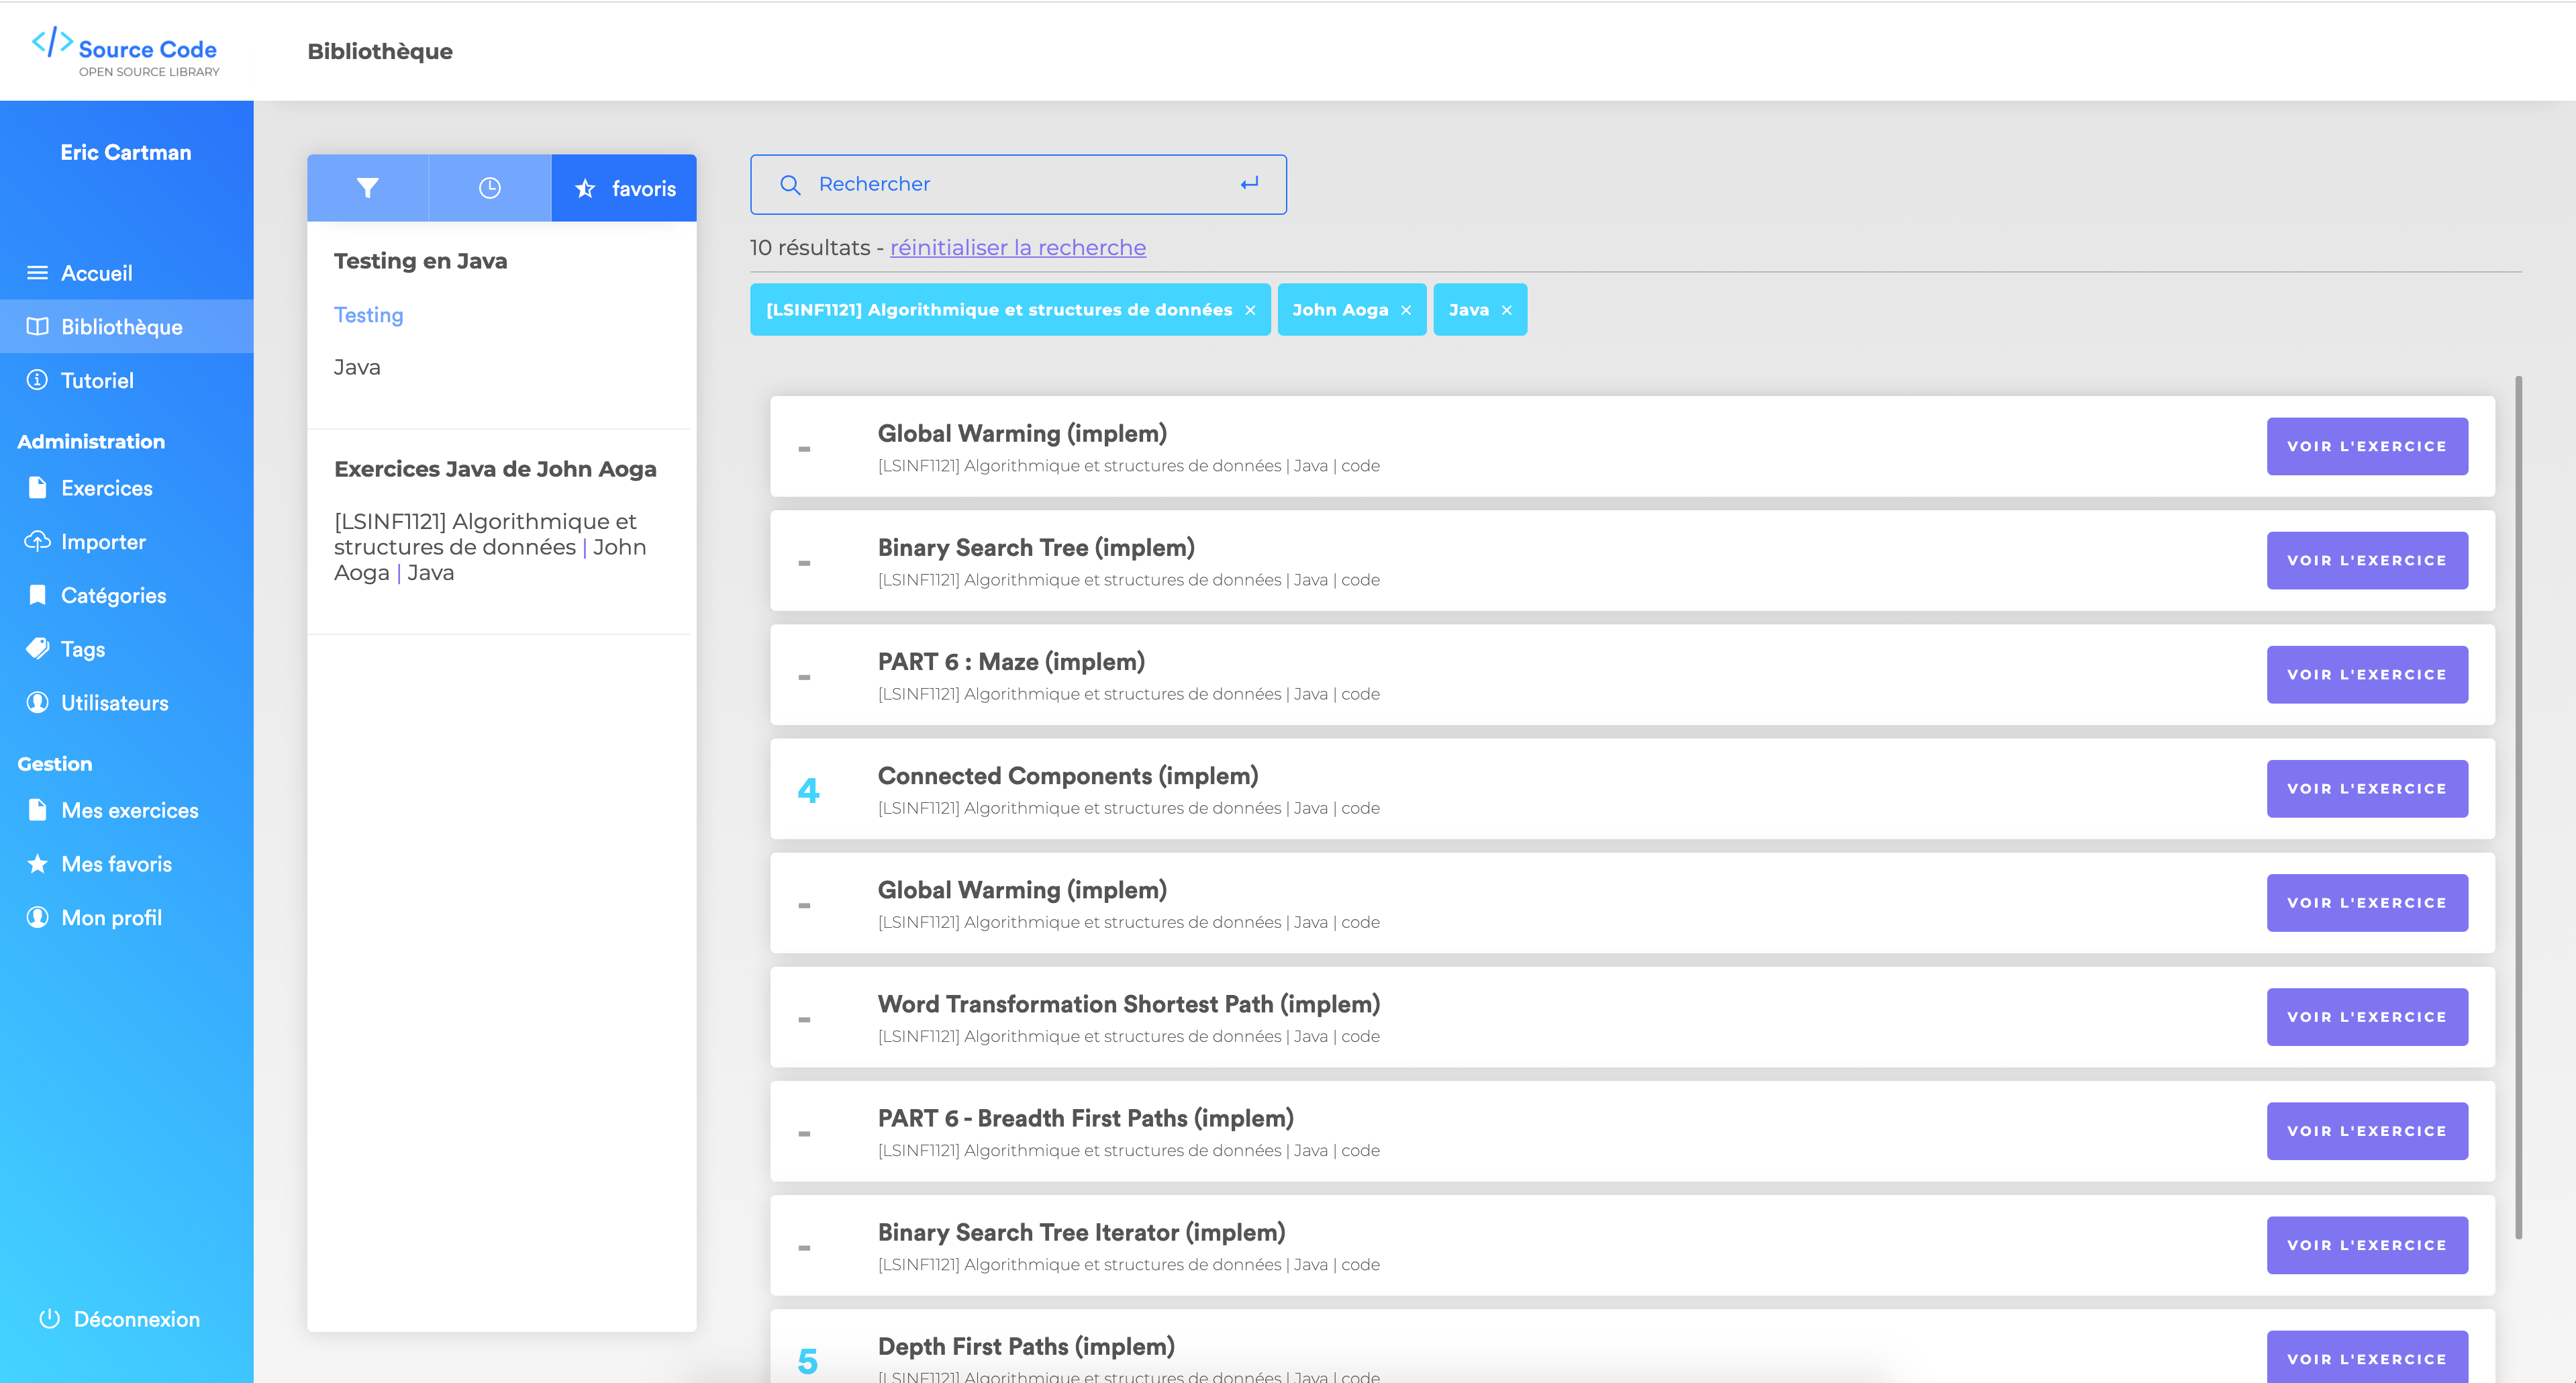
\includegraphics[width=\textwidth,height=\textheight,keepaspectratio]{images/client/favorite-panel.png}
    \centering
    \caption[SourceCode : le panneau "Favoris"]{Le panneau "Favoris"}
\end{figure}

Vous pouvez supprimer ou modifier les favoris depuis ce panneau en passant la souris sur un favori, puis en sélectionnant une des deux icônes qui s'affichent.

\begin{itemize}
    \item Le crayon permet de modifier le favori. Il mènera donc sur la page de modification de ce favori.
    \item La poubelle permet de supprimer le favori directement depuis le panneau.
\end{itemize}

Pour réinitialiser les critères de recherche, il faut cliquer sur "réinitialiser la recherche" juste en dessous du titre "Résultats de recherche".\\

\subsubsection{La \gls{fiche} d’une \gls{resinfo}}

Les \glspl{resinfo} sont le cœur de Source Code. Elles représentent toutes les contributions émises par la communauté. Elle peuvent être consultées depuis la bibliothèque en cliquant ensuite sur "voir l'exercice".\\

Voici à quoi ressemble la structure d'une \gls{fiche} :

\begin{figure}[H]
    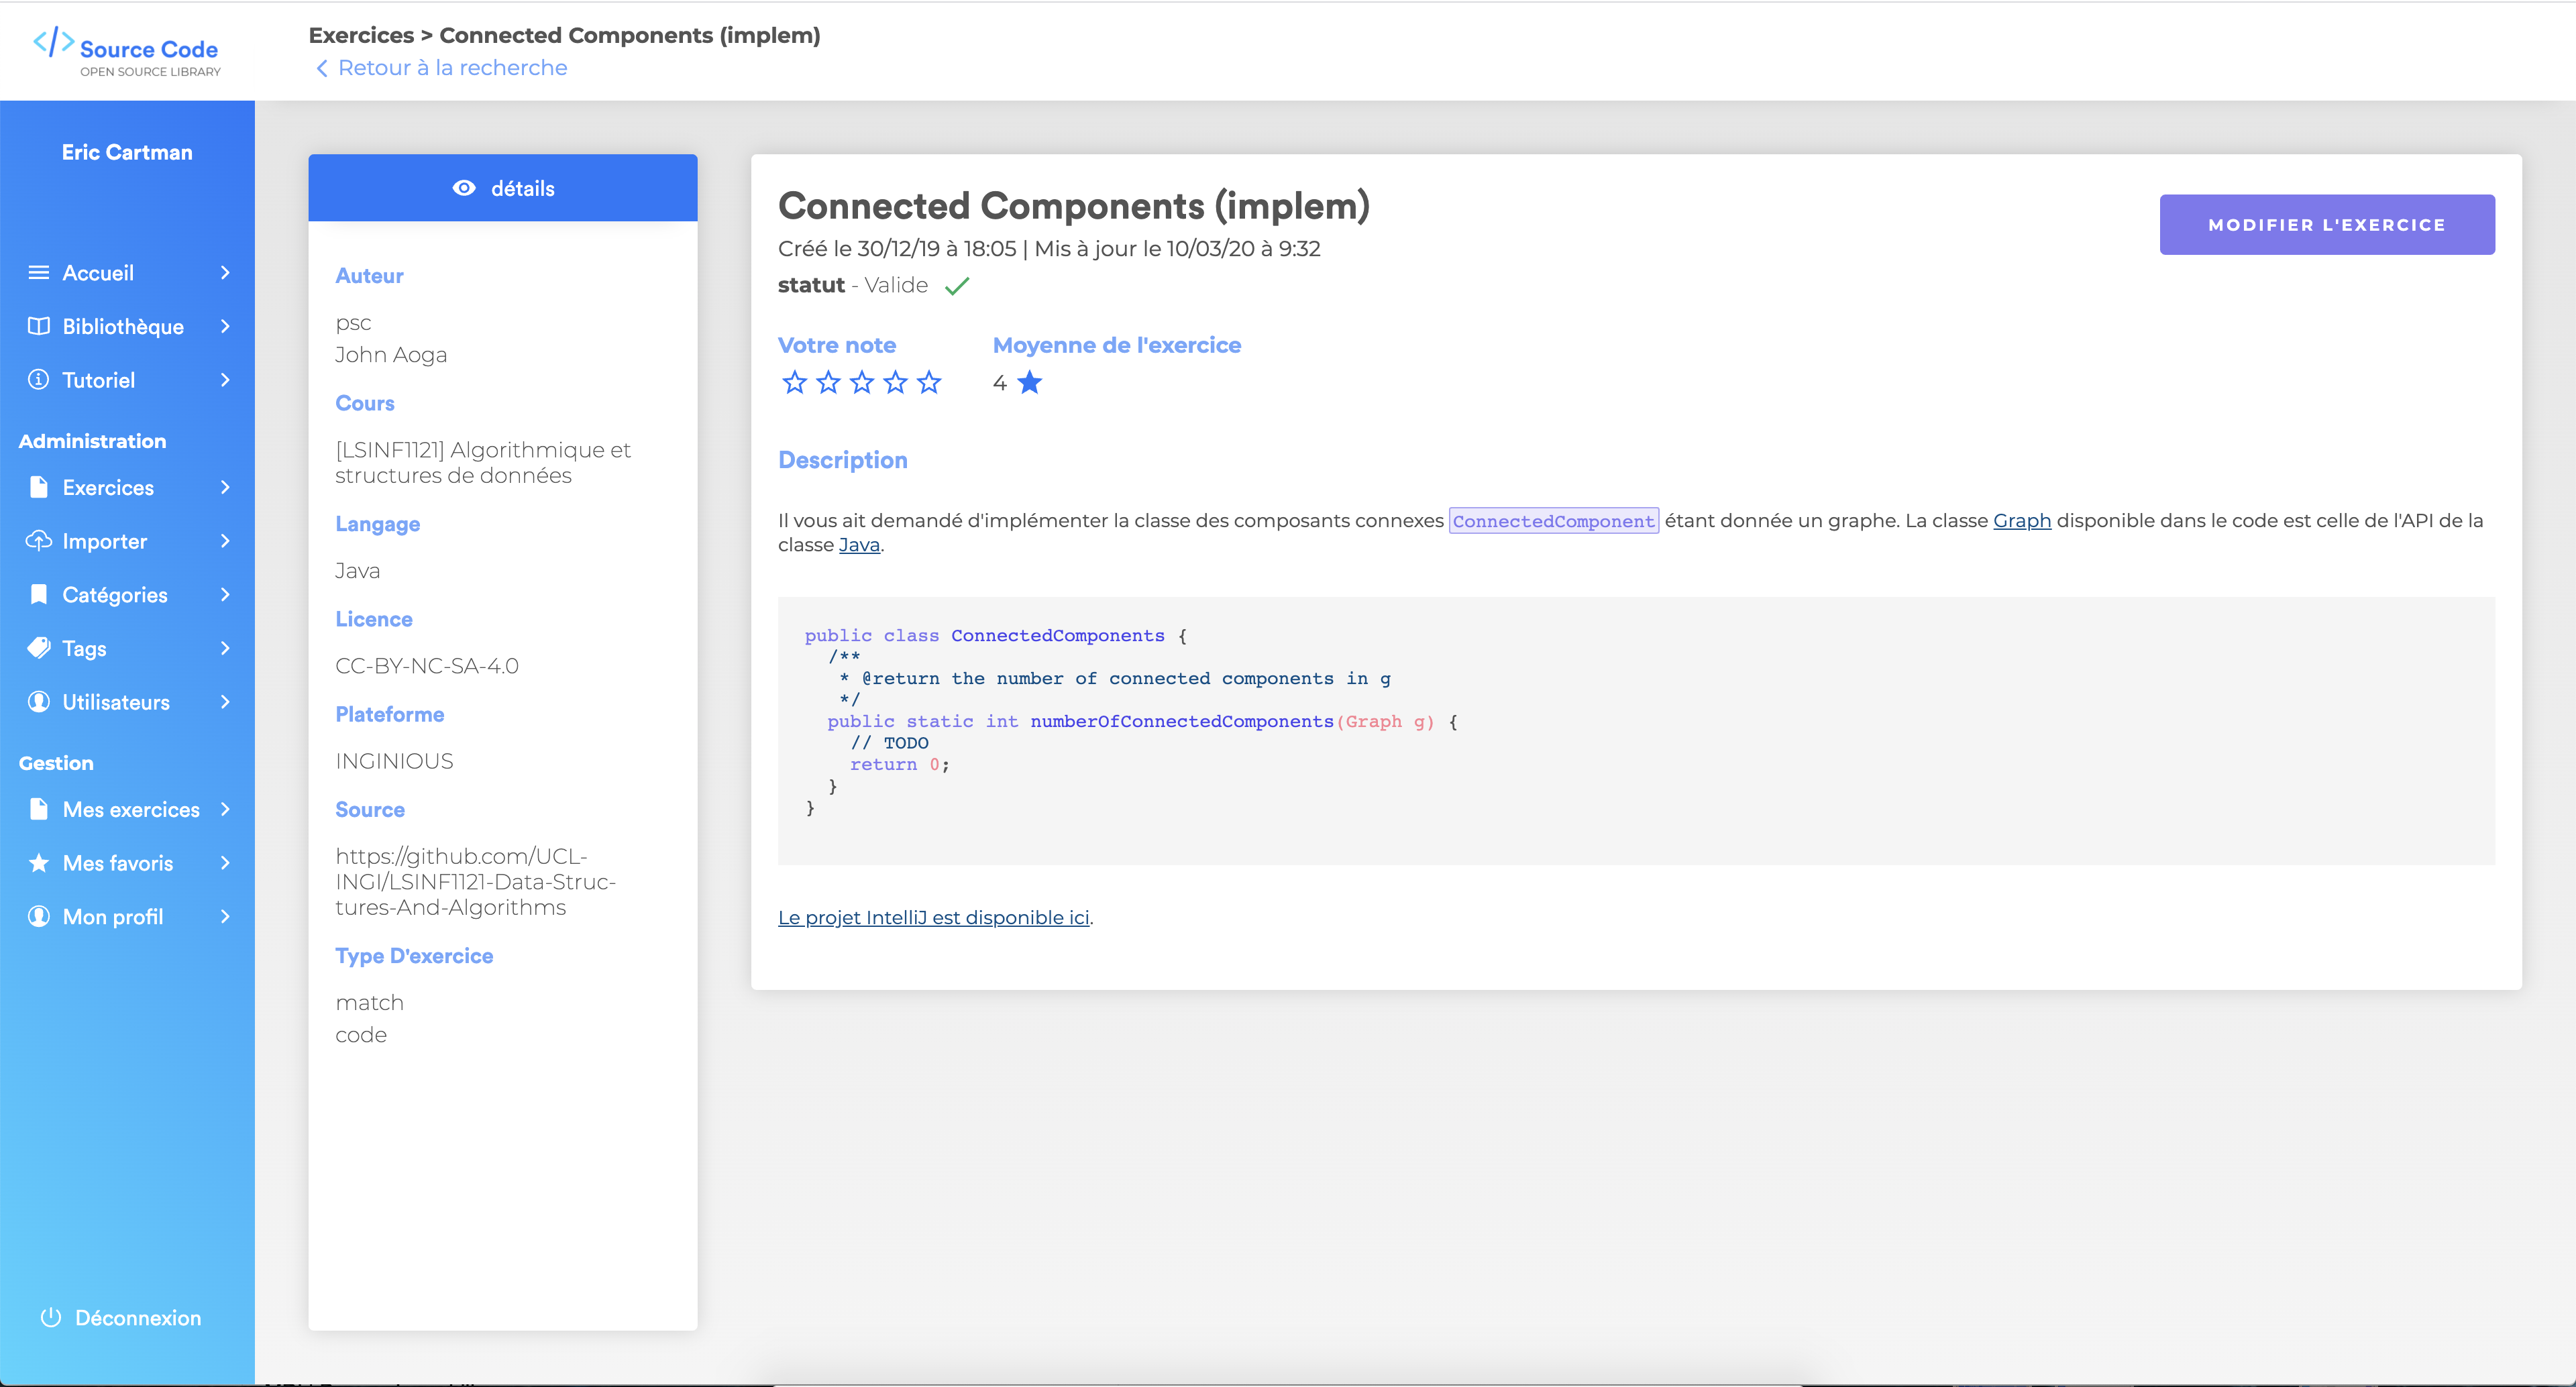
\includegraphics[width=\textwidth,height=\textheight,keepaspectratio]{images/client/fiche.png}
    \centering
    \caption[SourceCode : la représentation d'une \gls{fiche}]{la représentation d'une \gls{fiche}}
\end{figure}

\subsubsubsection*{\textit{Panneau de détails}}

Le panneau latéral contient tous les \glspl{tag} qui ont été ajoutés pour identifier la ressource. Plus il y en a, plus cette dernière sera favorablement référencée sur la plateforme. Chaque \gls{tag} est affiché sous une \gls{tagCat}.

\subsubsubsection*{\textit{\Gls{fiche} de la \gls{resinfo}}}

Sur la \gls{fiche} de la \gls{resinfo}, vous pouvez donner une note sur la qualité de la ressource sur 5 étoiles. Il suffit de cliquer sur une des étoiles pour donner un score (seulement si vous possédez un compte).\\

Lorsque la ressource vous appartient ou que vous êtes un administrateur, un bouton de modification apparait dans le coin supérieur droit de la \gls{fiche} de la ressource. Cliquer sur le bouton mènera sur le formulaire de modification de la ressource.\\

\subsection{Gestion}

Le module de gestion comprend :

\begin{itemize}
    \item La gestion de \glspl{resinfo} personnelles
    \item La gestion de favoris
    \item La consultation du profil
\end{itemize}

Ce module est accessible aux utilisateurs (possédant un compte) et aux administrateurs.

\begin{figure}[H]
    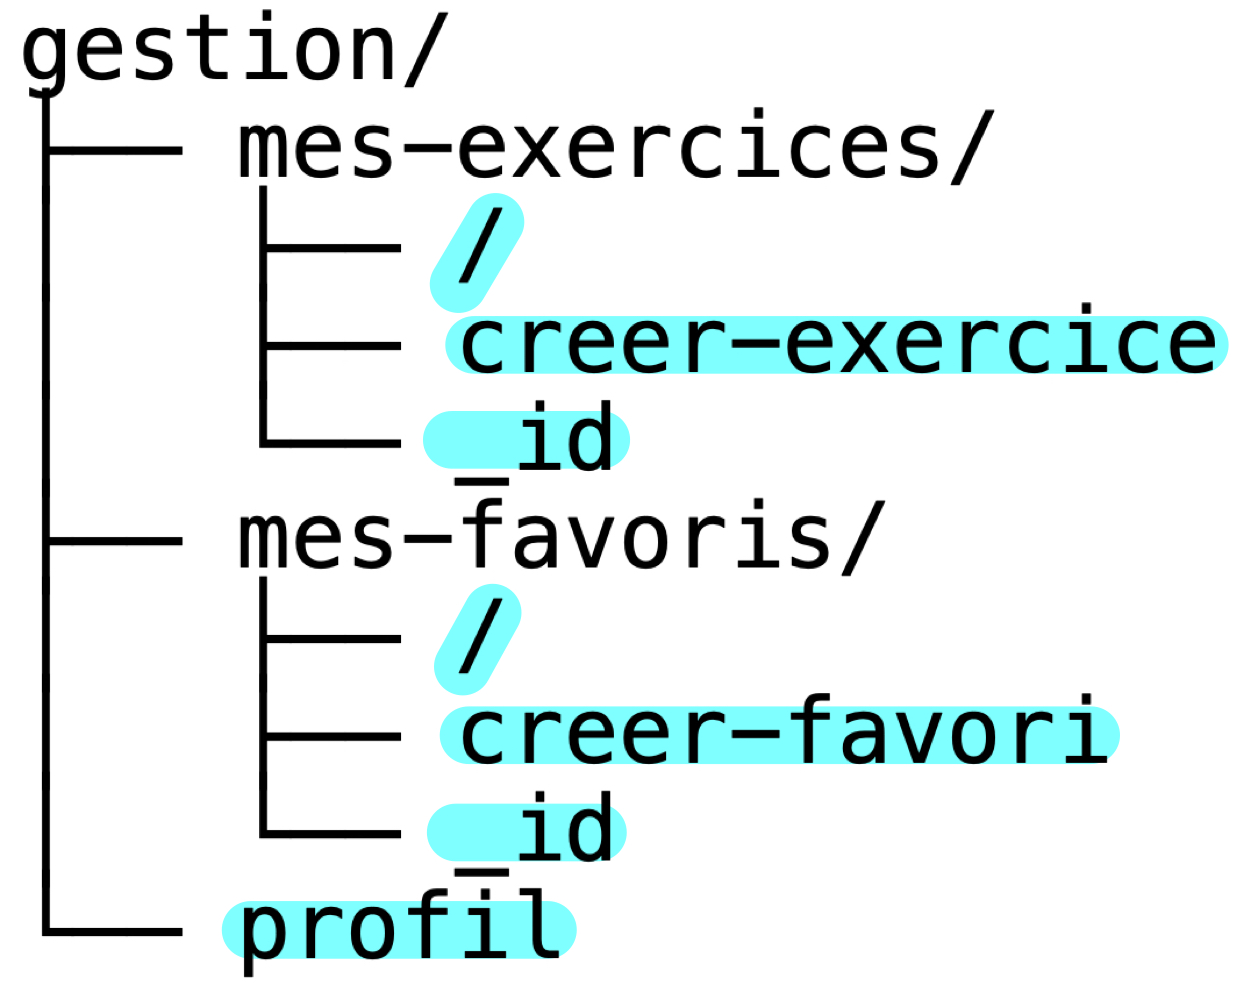
\includegraphics[width=\textwidth,height=\textheight,keepaspectratio]{images/client/gestion.jpeg}
    \centering
    \caption[SourceCode : module de gestion (url)]{Module de gestion (url)}
\end{figure}

\subsubsubsection{Gestion de \glspl{resinfo} personnelles}

La recherche fonctionne de la même manière que dans la bibliothèque, à la différence qu'elle est effectuée dans les \glspl{resinfo} personnelles seulement. Pour comprendre le fonctionnement du panneau à onglets, consultez la section \ref{section:panneau}.

\begin{figure}[H]
    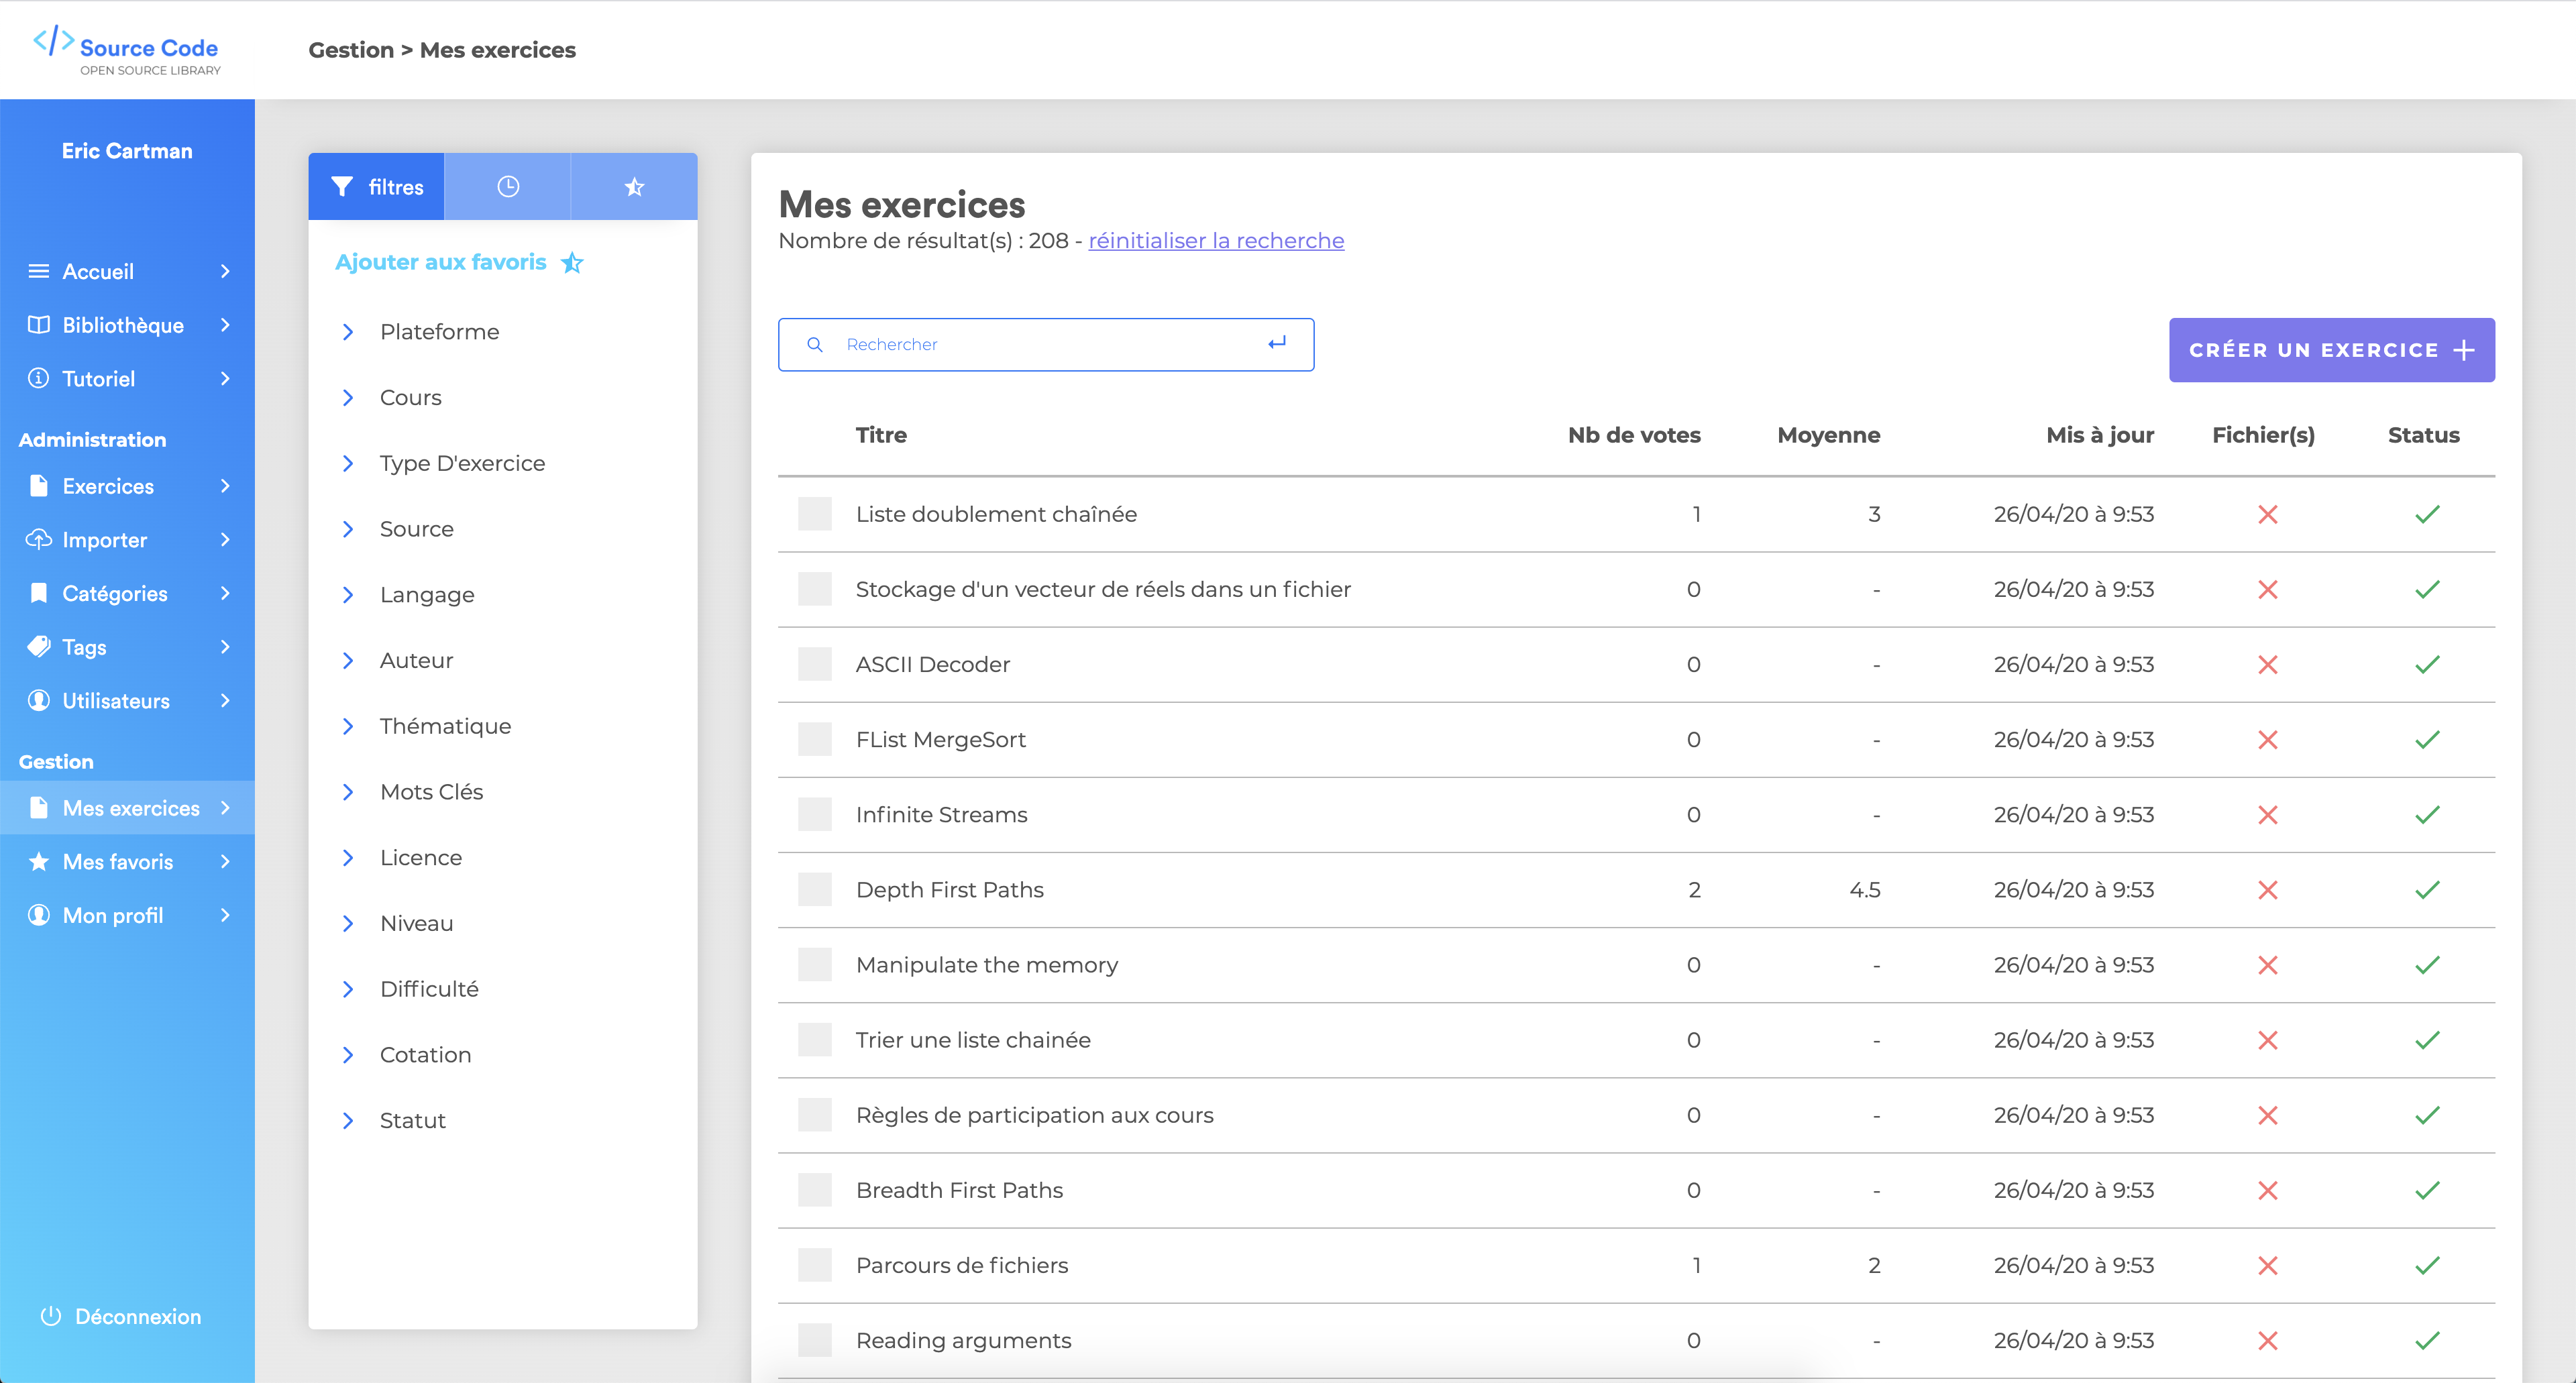
\includegraphics[width=\textwidth,height=\textheight,keepaspectratio]{images/client/gestion-exercices.png}
    \centering
    \caption[SourceCode : gestion des \glspl{resinfo} personnelles]{Gestion des \glspl{resinfo} personnelles}
\end{figure}

Plusieurs informations sont disponibles pour identifier les ressources informatiques :

\begin{itemize}
    \item Le titre de la ressource
    \item Le nombre de votes émis par la communauté
    \item La moyenne (sur 5) des votes émis par la communauté
    \item La date de mise à jour de la ressource informatique
    \item La présence d'une archive zip pour la ressource informatique
    \item Le statut de la ressource
\end{itemize}


\subsubsubsection*{\textit{Statuts d'une \gls{resinfo}}}

Voici les différents états que peuvent prendre la \gls{resinfo} :

\begin{itemize}
    \item 
\includegraphics[scale=0.3]{images/client/draft.png} \textbf{Brouillon}
    \begin{itemize}
        \item Signifie que la ressource n'est pas encore prête à être validée par l'administration. La ressource n'est donc pas disponible depuis la bibliothèque.
    \end{itemize}
    \item 
\includegraphics[scale=0.3]{images/client/pending.png} \textbf{En attente de validation}
    \begin{itemize}
        \item La ressource est mise en attente pour révision. Un administrateur se chargera de la valider ultérieurement.
    \end{itemize}
    \item 
\includegraphics[scale=0.3]{images/client/validated.png} \textbf{Valide}
    \begin{itemize}
        \item Lorsque la ressource est acceptée par l'administration, la ressource est alors validée et disponible publiquement dans la bibliothèque.
    \end{itemize} 
    \item 
\includegraphics[scale=0.3]{images/client/not-validated.png} \textbf{Invalide}
    \begin{itemize}
        \item Lorsque la ressource n'est pas considérée comme valide (mauvaise qualité d'écriture, doublons, incohérences), l'administrateur se réserve le droit d'invalider la ressource. Elle pourra néanmoins être modifiée pour la refaire passer en phase de révision.
    \end{itemize}
    \item 
\includegraphics[scale=0.3]{images/client/archive.png} \textbf{Archive}
    \begin{itemize}
        \item Quand une ressource est archivée, elle est alors uniquement accessible par les administrateurs et par son créateur.
    \end{itemize}
\end{itemize}

\subsubsubsection*{Gestion du statut de la ressource}

Pour modifier l'état d'une ou plusieurs ressources, il faut dans un premier temps les cocher. Une liste déroulante d'actions apparaitra à côté du bouton de création d'exercices avec les options suivantes :

\begin{itemize}
    \item Publier (envoyer pour révision)
    \item Mettre en brouillon
    \item Archiver
\end{itemize}

\begin{figure}[H]
    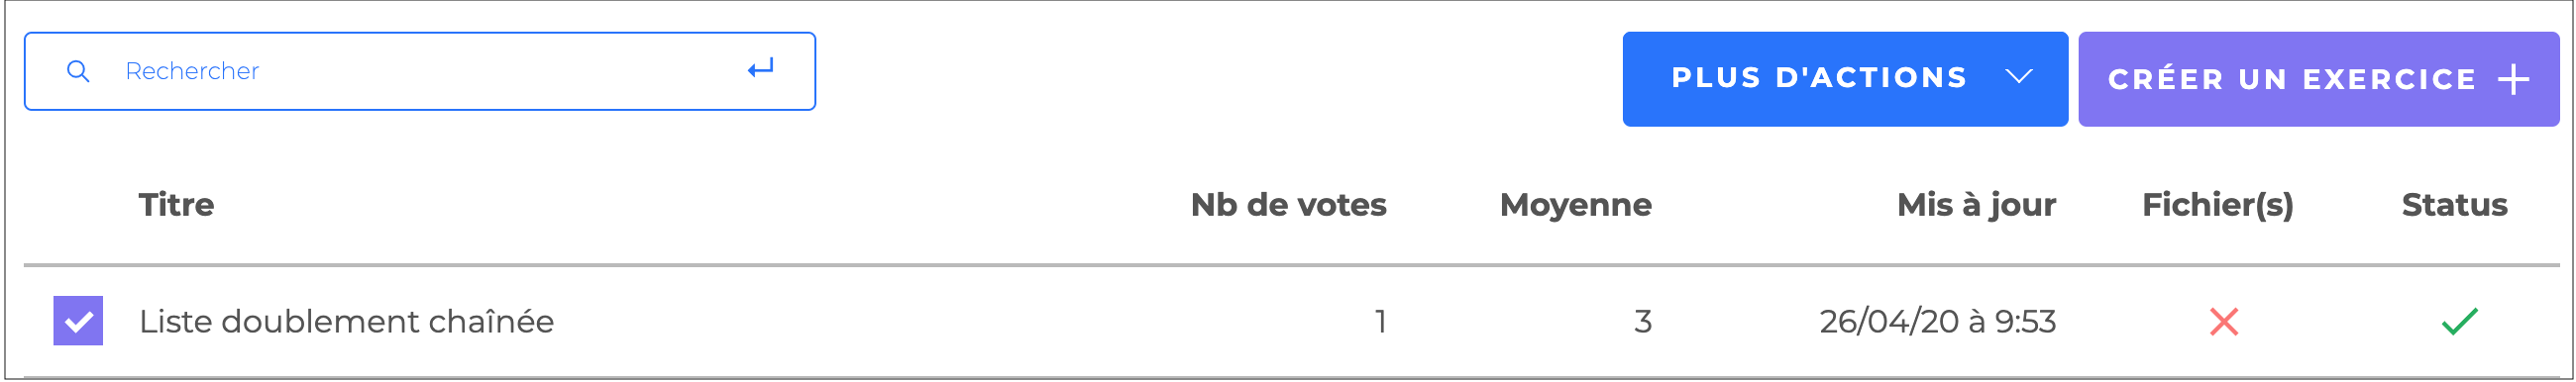
\includegraphics[width=\textwidth,height=\textheight,keepaspectratio]{images/client/gestion-options.png}
    \centering
\end{figure}

\subsubsubsection{Gestion de favoris}

\subsubsubsection{La consultation de profil}


\subsection{Administration}

\begin{figure}[H]
    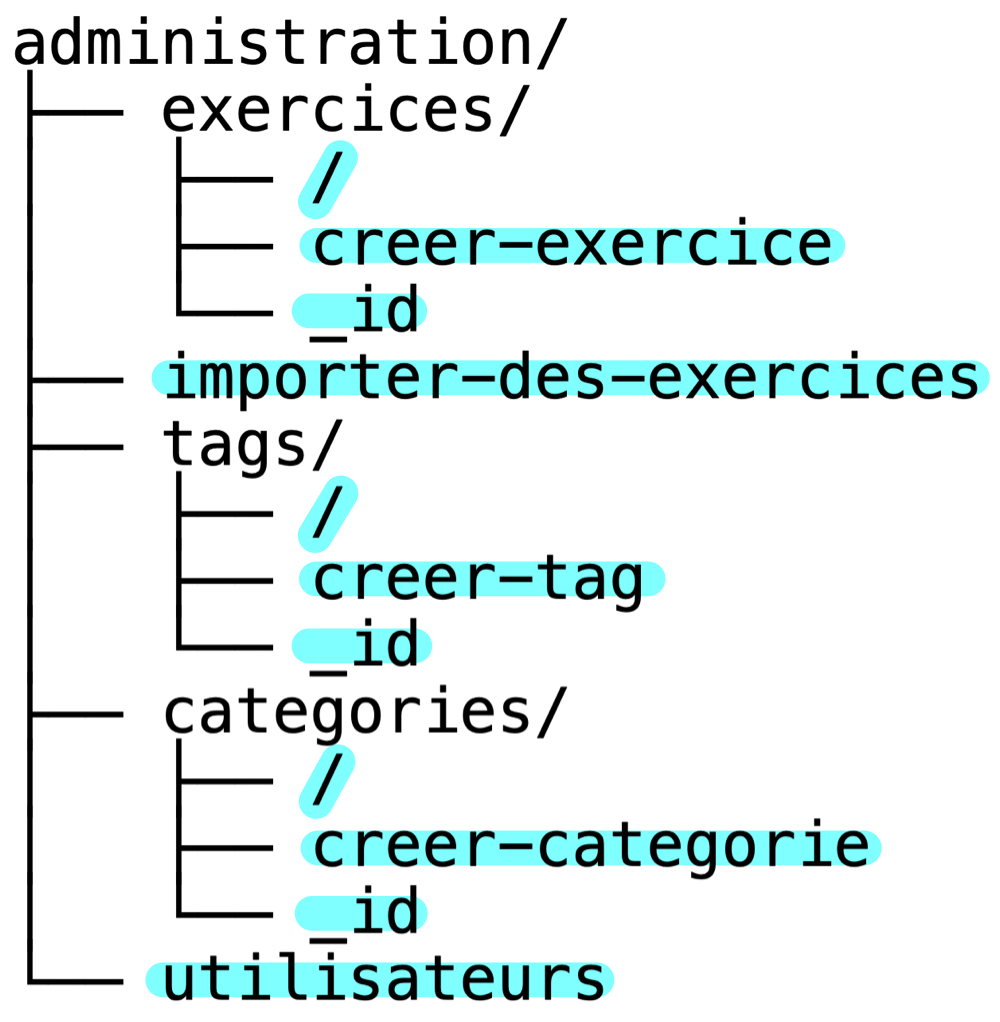
\includegraphics[width=\textwidth,height=\textheight,keepaspectratio]{images/client/administration.jpeg}
    \centering
    \caption[SourceCode : partie administration (url)]{Partie administration (url)}
\end{figure}


\subsection{Architecture}
% TODO : Je me doute que tu as ta propre manière d'aborder la chose ici, à toi de jouer ;)
% Pour moi, on doit y retrouver : 
% - des captures d'écrans montrant les principales fonctionnalités :
%    - recherche ( un exemple avec multi critères )
%    - création d'exercice
%    - la modération d'exercices par un admin ( la main page avec plusieurs)
% - avec les captures, des explications sur la conception des pages
% ( Par exemple, "Afin de résoudre les problèmes UX que nous avons constatés avec les autres plateformes, nous avons ...")
% - ETC 